\documentclass[12pt]{article}

%%%Package Manager%%%
\setlength{\parindent}{4em}

\usepackage{amsmath}
\usepackage{setspace}
\usepackage{fancyvrb}
\usepackage{graphicx}
\usepackage{geometry}
\usepackage{hyperref}

\geometry{letterpaper, portrait, margin=1in}
%%%%%%%%%%

%%%Title Page%%%
\title{
	\begin{center}
		
\includegraphics[scale=0.5]{uga.png}\\
 	\end{center}
 	CSEE 4320\_25 Mechatronics Systems Engineering
\bigbreak Lab 1 - Electronics Design Lab
}

\author{
{\normalsize
\begin{tabular}{l c c}
& \textbf{Zachary Davis} & \\
& 811960668 & \\
\textbf{Category} & Zachdav@uga.edu & \\
\hline
Lab 1: Introduction to Lab Instruments & 20\% & \\
Lab 2: Introduction to Computer Systems & 25\% & \\
Lab 3: Tradeoffs Between Hardware \& Software & 25\% & \\
Lab 4: Analog Input \& Output & 30\% & \\
\hline
\end{tabular}
}
}

\date{\bigskip
\today}
%%%%%%%%%%

%%%Content%%%
\begin{document}
	\maketitle
	\newpage
	
	\tableofcontents
	\newpage

	\section{Lab 1: Introduction to Lab Instruments}
		\subsection{A}
			\paragraph{}
				For the first part of lab one I am to build to following passive RC circuit on a breadboard.

				\begin{center}
					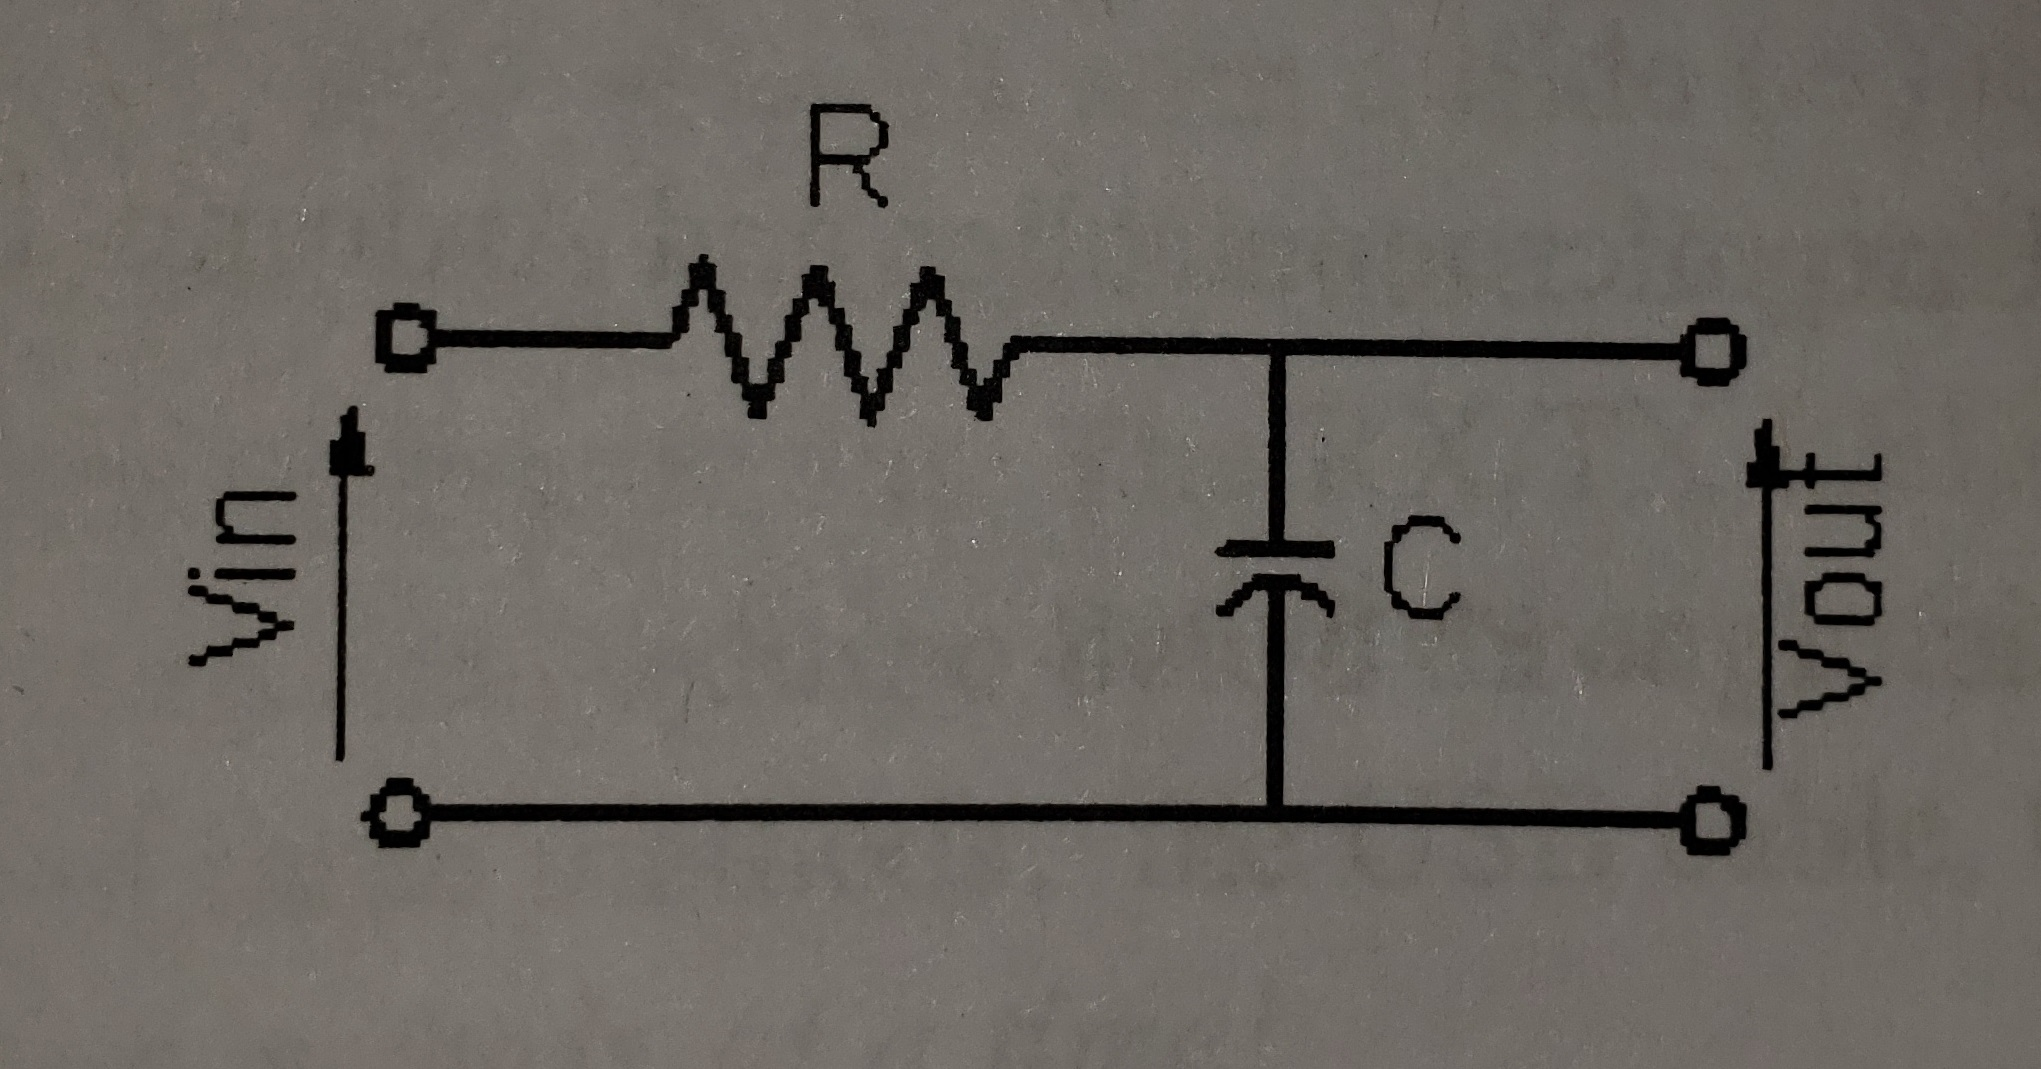
\includegraphics[scale=0.1]{1.jpg}\\
				\end{center}

		\subsection{B}
			\paragraph{}
				To build the above circuit I will be using a 10 kOhm resistor and a 1 uF capacitor.
		
		\subsection{C}
			\paragraph{}
				Before actually building the shown circuit I took the 10 kOhm resistor and used a multimeter to measure its resistance value 
				ten times and recorded the necessary statistical data below to describe its precision and accuracy.

				\begin{center}
					\begin{tabular}{ |c|c| }
						\hline
						\textbf{Resistance Measurements} & --- \\ 
						\hline
 						1 & 9.99 kOhms \\ 
						2 & 9.99 kOhms \\ 
						3 & 10.06 kOhms \\ 
						4 & 9.99 kOhms \\ 
						5 & 9.99 kOhms \\ 
						6 & 9.98 kOhms \\ 
						7 & 9.99 kOhms \\ 
						8 & 9.99 kOhms \\ 
						9 & 9.99 kOhms \\ 
						10 & 9.99 kOhms  \\ 
						Average & 9.996 \\
						Standard Dev & 0.066\\
						Precision & 9.996+/-0.066\\
						Percent Accuracy & 0.04\% \\
						\hline
					\end{tabular}
				\end{center}

		\subsection{D}
			\paragraph{}
				For this part of the lab I needed to determine the value of the time constant, $\tau$, using the first order differential equation 
				and the cut0ff frequency of our specific low pass filter.

				\begin{equation}
					V_{Out} = V_{In}*\frac{X_{C}}{\sqrt{R^2+X_C^2}}\\
				\end{equation}
				\begin{equation}
					where, X_C = \frac{1}{2 \pi fC}
				\end{equation}

				\begin{equation}
					f_C = \frac{1}{2 \pi \tau}\\
				\end{equation}
				\begin{equation}
					where, \tau = RC
				\end{equation}
				\begin{equation}
					\tau = 0.01 uS===>f_C = 15.916 Hz
				\end{equation}
				For our specific passive low pass filter the cut off frequency is 15.916 Hz and any frequencies lower than this will be able to pass 
				through to Vout.

		\subsection{E}
			\paragraph{}
				Since we now the value of $\tau$ we can calculate the rise time of this RC circuit...
				\begin{equation}
					t_r = \frac{\tau}{2 \pi f}
				\end{equation}
				\begin{equation}
					t_r = \frac{0.0157}{Bandwidth}
				\end{equation}
				We also now that the frequency cutoff is equal to the bandwidth therefore...
				\begin{equation}
					t_r = 0.000987\tau
				\end{equation}
				For the settling time we need...
				\begin{equation}
					T_s = -\frac{ln(tolerance)}{damping*frequency}
				\end{equation}
				For our particular circuit the 5\% settling time is...
				\begin{equation}
					T_s = 0.03 uS
				\end{equation}
				Finally for the input frequency in the physical circuit I input 10 Hz sine wave and $\tau$ with the measured value do not perfectly match.  
				This is most likely because the circuit elements are none ideal from the resistor and capacitor all the way to the slight resistance in the 
				function generator itself.  Below I have included the image from the oscilloscope and graph of the data retrieved from the oscope in 
				excel.

				\begin{center}
					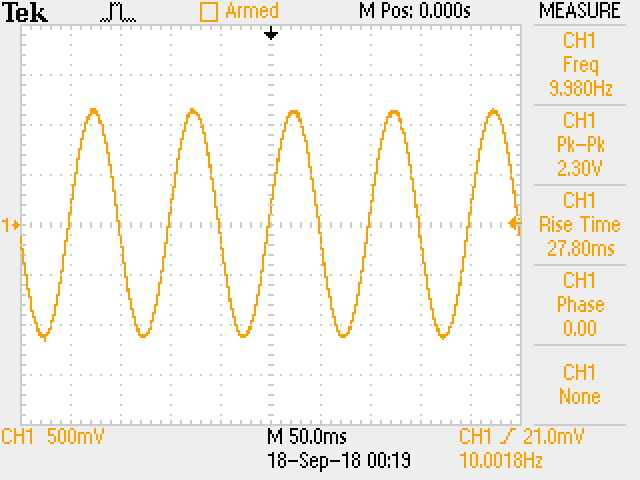
\includegraphics[scale=0.6]{output.jpg}\\
					\vspace{1cm}
					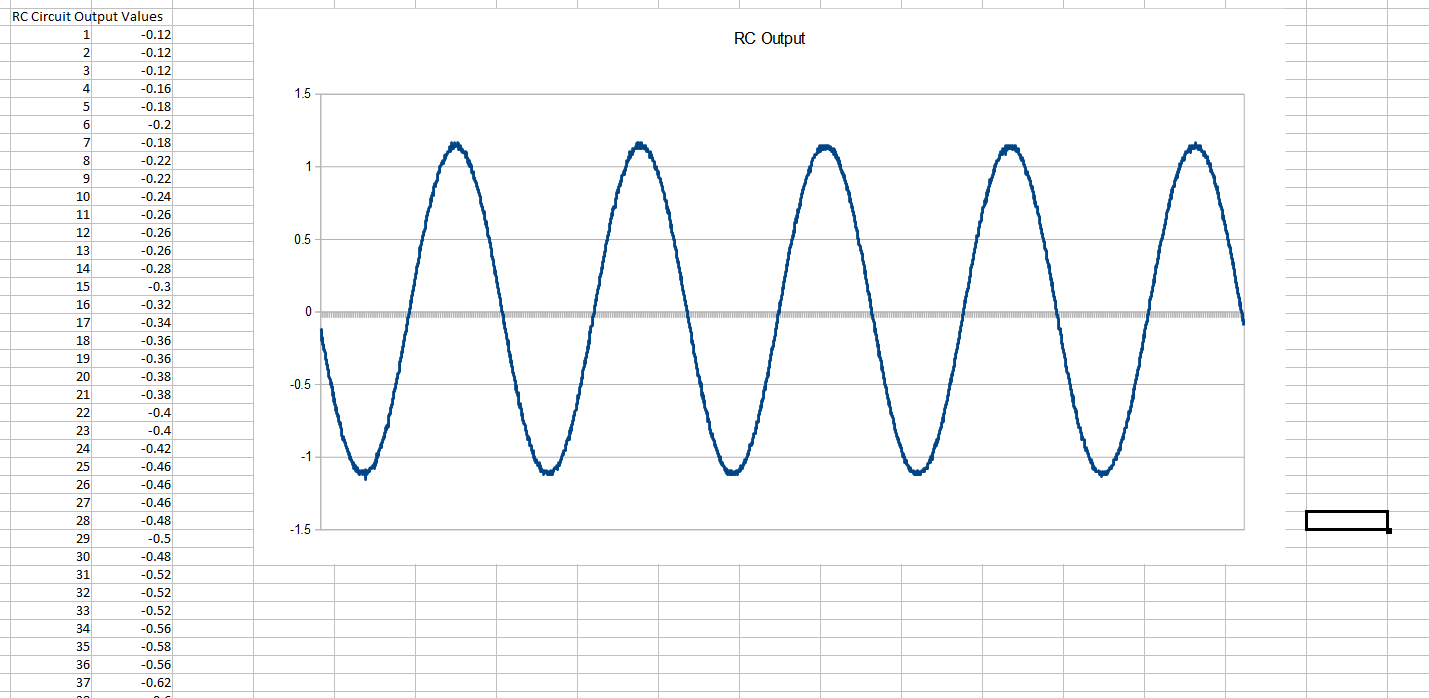
\includegraphics[scale=0.15]{eoutput.png}
				\end{center}
		
		\subsection{F}
			\paragraph{}
				For this section I used the same 10 Hz input that I used in the previous portion of the lab.  The input and output for this circuit should
				theoretically be 90 degrees out of phase and the magnitude ratio should be equal to 1 - the voltage drop of our resistor which in this
				case is 10 kOhms.  Again like in the previous section the output of the RC circuit is similar to what expected but not ideal and again this is
				because all of the circuit elements being used are not ideal and they all propagate into the difference we see.  I included the image from 
				the oscope below as well as the data collected and graphed in excel.

				\begin{center}
					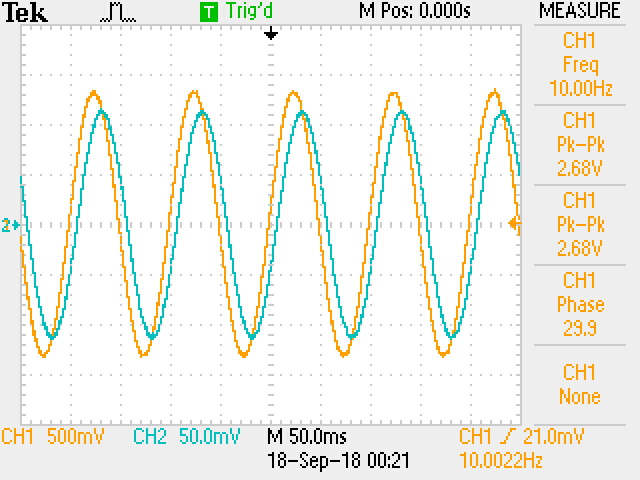
\includegraphics[scale=0.6]{input.jpg}\\
					\vspace{1cm}
					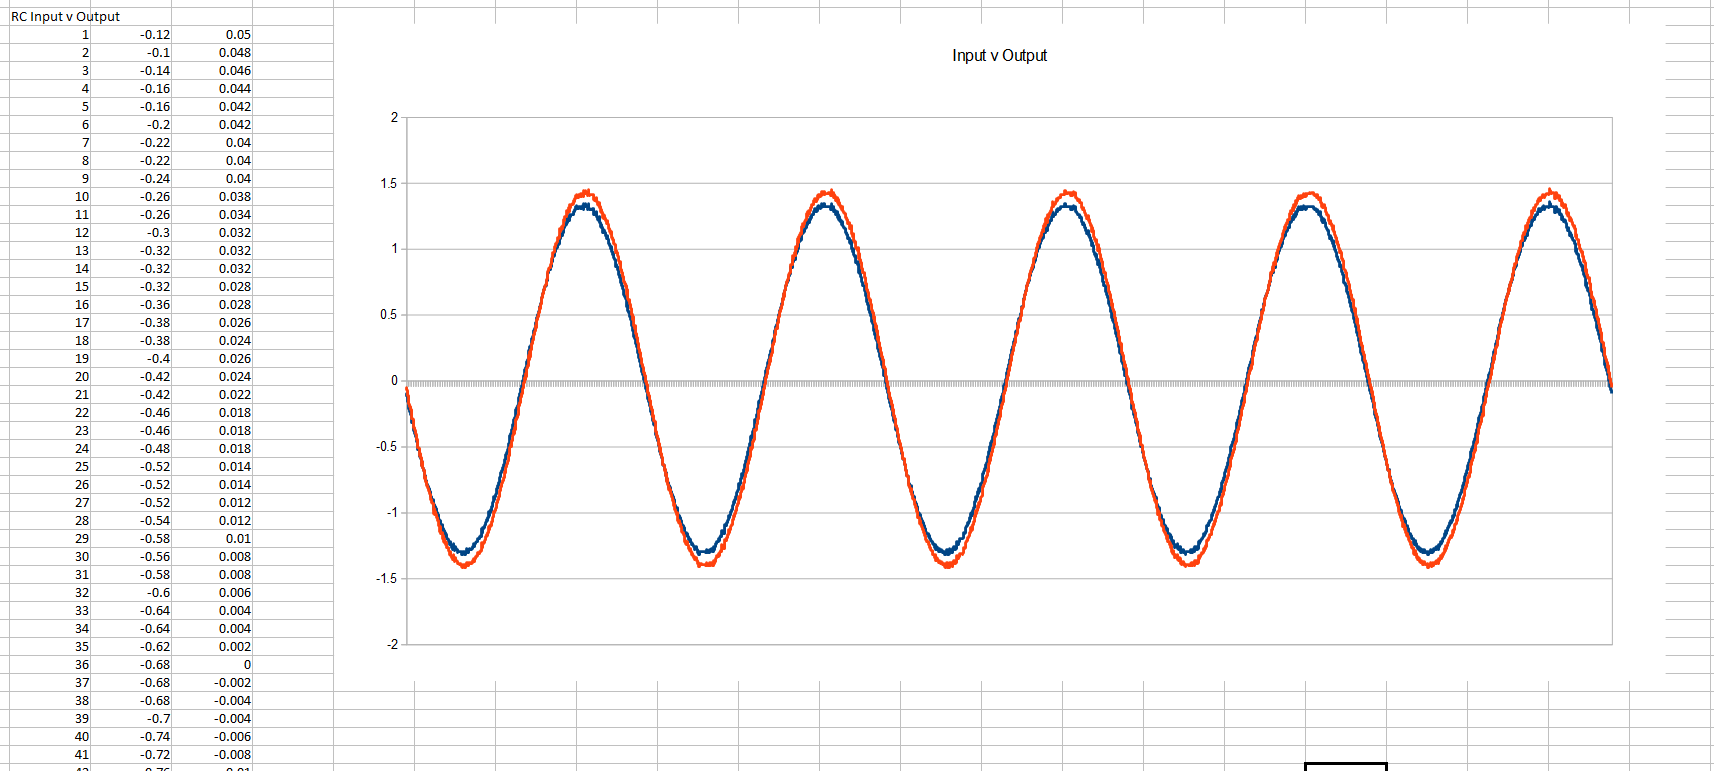
\includegraphics[scale=0.15]{einput.png}
				\end{center}

		\subsection{G}
			Below i have included the image from the oscope that performed the FFT option with both the input and output signals from the previous port of
			this lab below.
			
			\begin{center}
				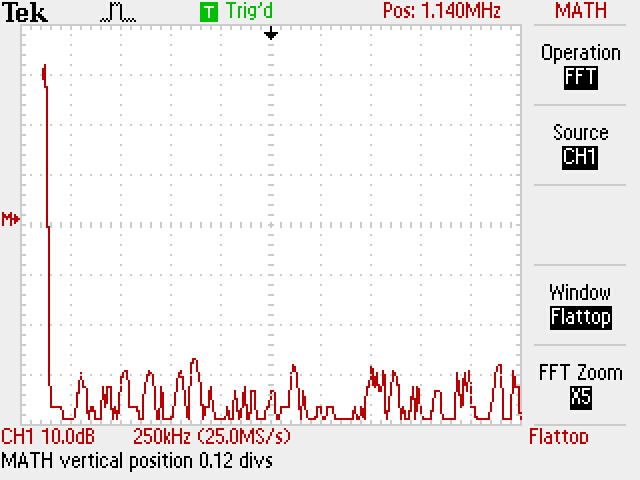
\includegraphics[scale=0.6]{fft1.jpg}\\
				\vspace{1cm}
				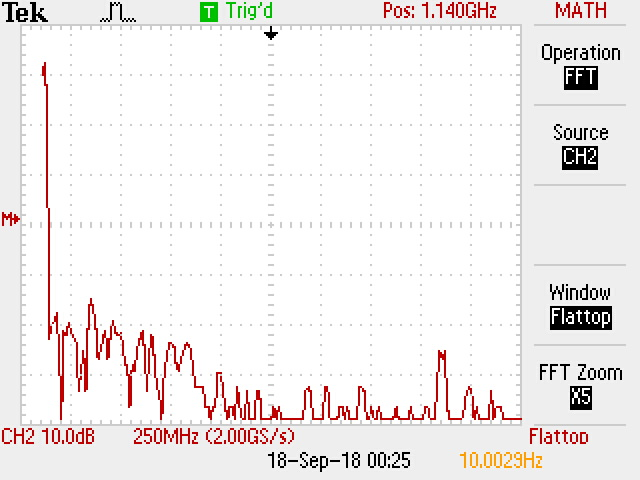
\includegraphics[scale=0.6]{fft2.jpg}\\
				\vspace{1cm}
				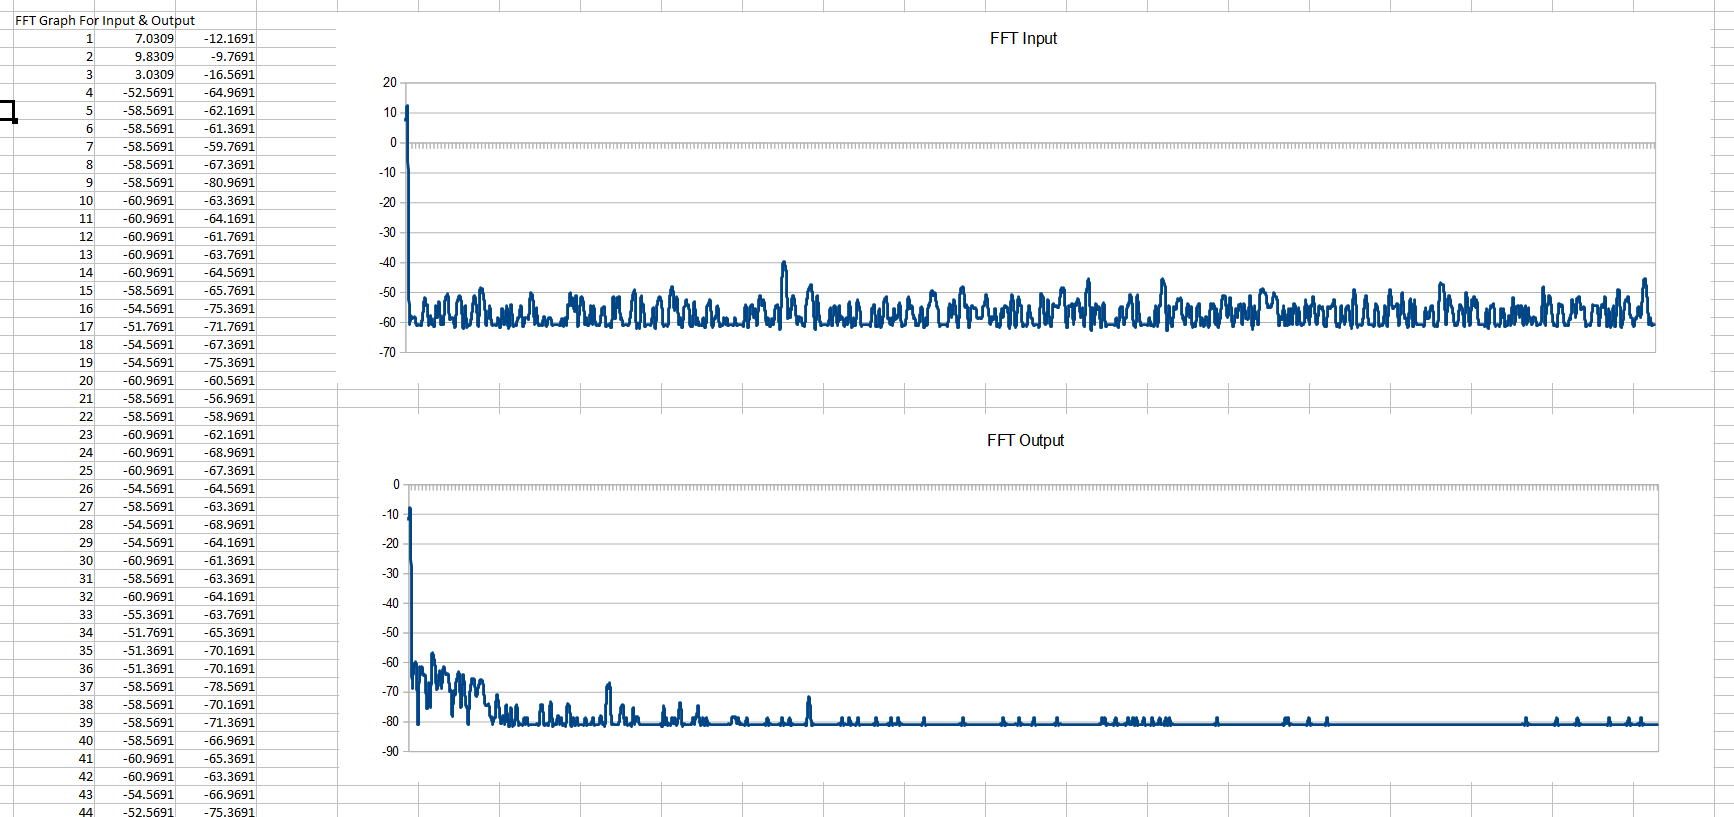
\includegraphics[scale=0.15]{efft.png}
			\end{center}

	\section{Lab 2: Introduction to Computer Systems}
		\subsection{Blinking LED}
			\subsubsection{A}
				\paragraph{}	
					For this part of the lab we are being introduced to the arduino and modifying sample code to practice.  I took the blink code and 
					modified it so that the pin being used to output is now pin 12 and changed the delay such that it is high for 0.5 seconds and low
					for 1.5 seconds.  Finally i rewrote all of the line by line comments to show my understanding of what is happening.  Below is the final
					code that was compiled for the arduino.

					\begin{center}
						\begin{verbatim}
							/*
							Blink
							Turns on an LED on for one second, then off for one second, repeatedly.

  							Most Arduinos have an on-board LED you can control. On the Uno and
  							Leonardo, it is attached to digital pin 13. If you're unsure what
  							pin the on-board LED is connected to on your Arduino model, check
  							the documentation at http://www.arduino.cc

  							This example code is in the public domain.

  							modified 8 May 2014
  							by Scott Fitzgerald
 							*/

 							/*
  							*  Modified by: Zachary Davis
  							*/

							//This is the none looping portion of arduino code used for one
							//time initialization.
							void setup() {
 								//Initialize Pin 12 as the output pin.
 			 					pinMode(12, OUTPUT);
							}

							//The inifinite looping portion of the arduino program.
							void loop() {
  								//Set pin 12 to output logic high
  								digitalWrite(12, HIGH); 
  								//Wait for 0.5 seconds  
  								delay(500);         
  								//Set pin 12 to output logic low     
  								digitalWrite(12, LOW);
  								//Wait for 1.5 seconds    
  								delay(1500);              
							}
						\end{verbatim}
					\end{center}
			
			\subsubsection{B}
				\paragraph{}
					This section of the lab is just the uploading of the previous code onto the actual board, which was successful.

			\subsubsection{C}
				\paragraph{}
					Now I built a circuit that connected pin 12 to a resistor and led in series to demonstrate the program.  We needed a 
					current limiting resistor for the led and given that the output voltage is 5V and we are connecting to one led and we 
					desire a current some from 20 - 30 mA we are using a 270 Ohm resistor.  Below I have included a diagram of the circuit
					I have constructed.

					\begin{center}
						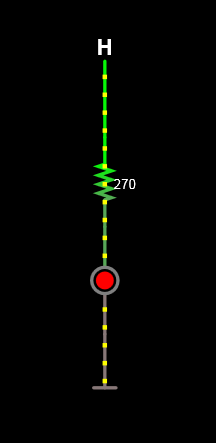
\includegraphics[scale=0.3]{circuit1.png}\\
					\end{center}

			\subsubsection{D}
				\paragraph{}
					This program does work as expected and a picture of the circuit with the arduino is included below.
				
					\begin{center}
						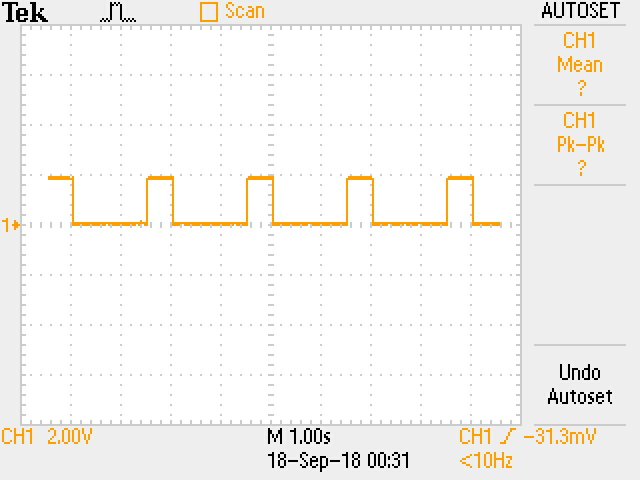
\includegraphics[scale=0.6]{oblink.jpg}\\
						\vspace{1cm}
						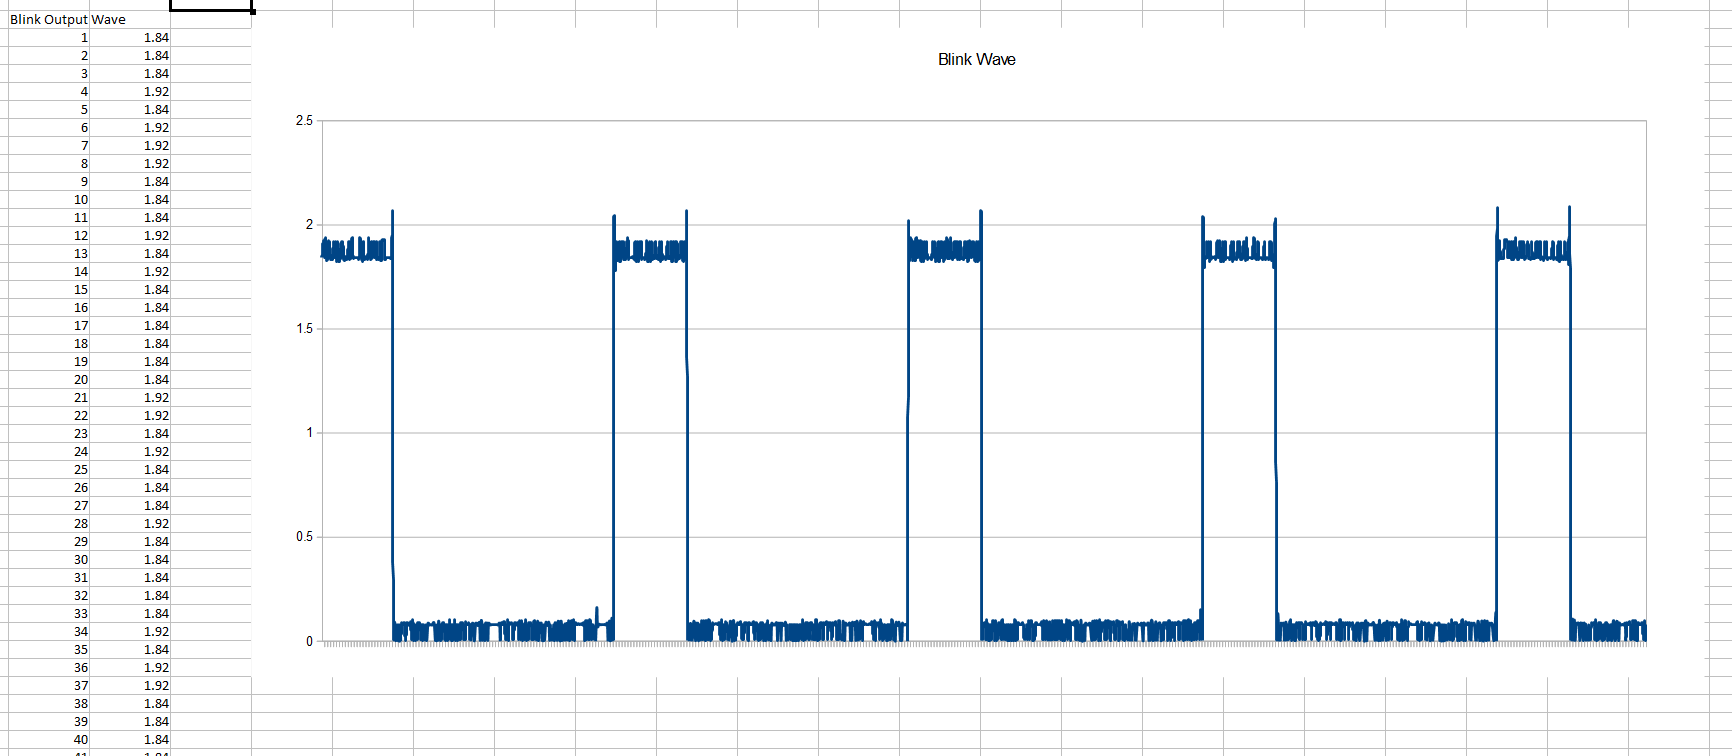
\includegraphics[scale=0.15]{eblink.png}\\
					\end{center}

			\subsubsection{E}
				\paragraph{}
					For me, i can no longer see the led blinking around 60 - 80 Hz, which makes since because that approaches the refesh rates
					of many led displays.  This waveform being a digital output is a square wave with a peroid being 0.5 seconds high and 1.5
					seconds low.

		\subsection{Pull-Up \& Pull-Down Resistors}
			\paragraph{}
				For this part of the lab we are instructed to build the circuit below connecting the logic gate to pin 12 on the arduino and using the arduino's 5V and 
				ground pins.  I also modified the blink code from earlier further by changing the on time to 1 second and the off time to 0.5 seconds.  Below you can 
				see the physical circuit and the waves from the collector and base of the transistor.

				\begin{center}
					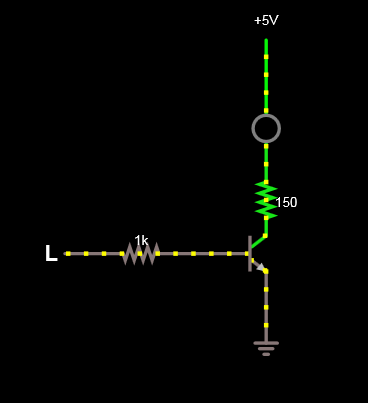
\includegraphics[scale=0.4]{pull-up.png}\\
					\vspace{1cm}
					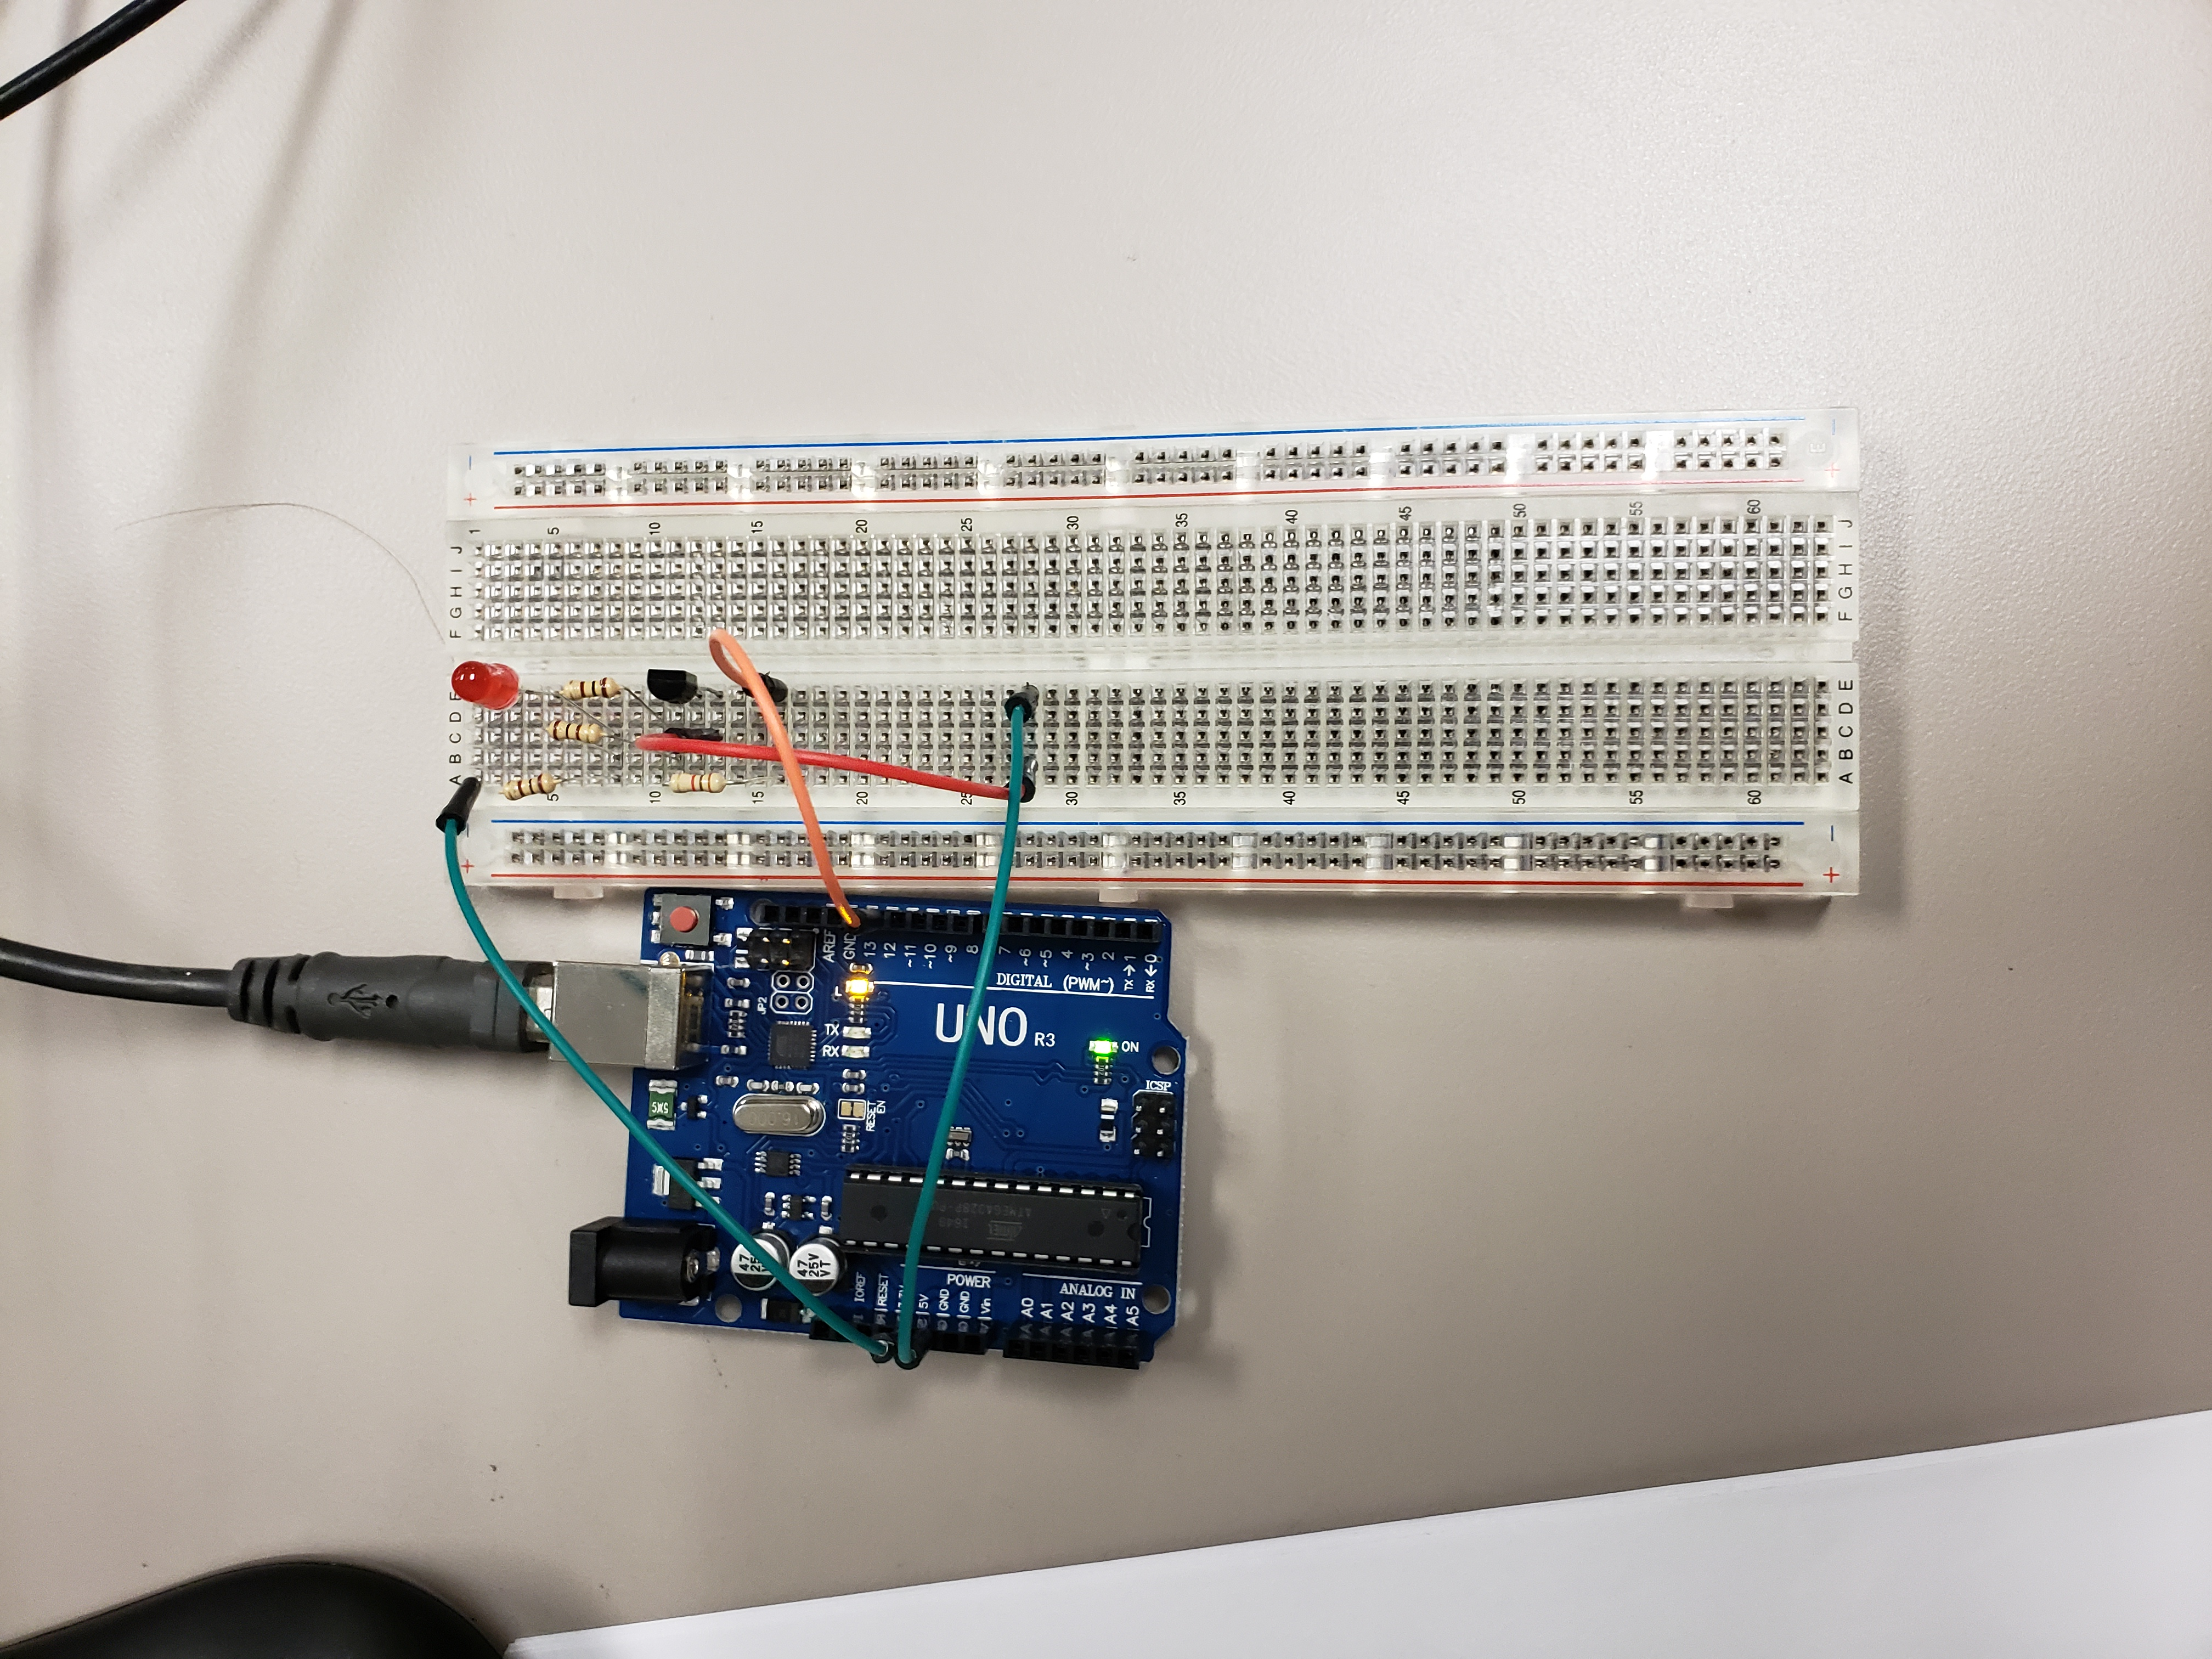
\includegraphics[scale=0.03]{transistor.jpg}\\
					\vspace{1cm}
					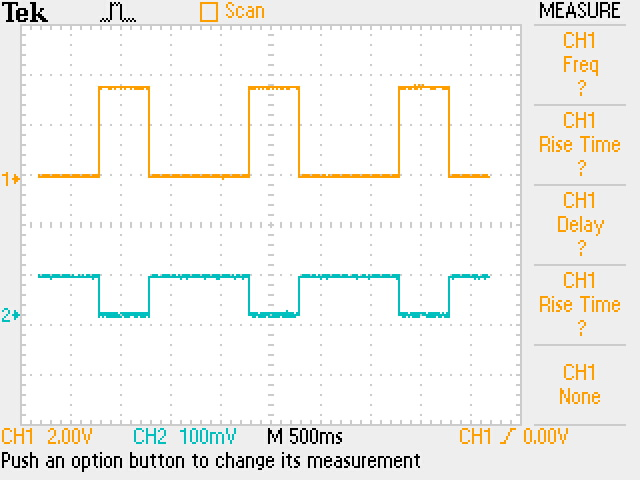
\includegraphics[scale=0.5]{otransistor.jpg}\\
				\end{center}

			\subsubsection{A}
				\paragraph{}
					The voltage across this wire will not be 0 or 5 volts across its length but it will be difficult to predict the voltage acorss this wire.  In order
					to be sure that the voltage is 0 or 5 volts it needs to be connected to ground or a power supply.  Essencitally the wire is at a floating point
					were we are unable to predict its voltage and it is pull-up and pull-down resistors that solve this issue.
			
			\subsubsection{B}
				\paragraph{}
					For a pull-up resistor as the name suggests the output is pulled high when the switch is open and low when the switch is closed all due to the 
					flow of current.

			\subsubsection{C}
				\paragraph{}
					Without the pull-up resistor it would be difficult to say what the voltage at DI would be.  Like i mentioned earlier it would be at this floating point
					where we are unable to predict what the voltage would be.

			\subsubsection{D}
				\paragraph{}
					The pull-down resistor is the polar opposite of the pull-up resistor.  Again as its name suggests when the pull-down switch is open the output is
					pulled down to a logical low and when the switch is closed then the output is logic high because current can flow from VCC to DI.

			\subsubsection{E}
				\paragraph{}
					Without the pull-down resistor it would be difficult to say what the voltage at DI would be.  Like i mentioned earlier it would be at this floating point
					where we are unable to predict what the voltage would be.

			\subsubsection{F}
				\paragraph{}
					The pull-up and pull-down resistors are very important when dealing with conveying digital signals because they can be used as very effective 
					logic gates forcing the values to be very predictable logic low and logic high values.

		\subsection{Transistors}
			\subsubsection{A}
				\paragraph{}
					Looking at the oscope the delay time and rise time of the transistor or the turn on time is 0.  I am refering to the below image.
			
			\subsubsection{B}
				\paragraph{}
					Again refering to the image above the storage time or the fall time of the transistor or the turn off time is 0.

			\subsubsection{C}
				\paragraph{}
					Yes they most certainly are looking at the output of the oscillosope.

			\subsubsection{D}
				\paragraph{}
					The current applied to the base of the transistor when the output of the arduino at pin 12 is high is 4.32 mA, which is most 
					certainly within the arduino's specification.

			\subsubsection{E}
				\paragraph{}
					If you were to remove the current limiting resistor to the base what would happen is that when the arduino pin 12 outputs high a 
					massively high current would be reached and flow through the base which would damage the transistor and the led.

			\subsubsection{F}
				\paragraph{}
					In theory the voltage drop across the led should be 1.9 V and in practice it is with an acceptable range.  When the led is on it has a 
					voltage drop of 2.03 V.
			
			\subsubsection{G}
				\paragraph{}
					When the arduino pin 12 is high current will flow from the 5 V Vcc through the led then that current will flow into the collector along with 
					the current from the pin 12 flowing into the base.  Finally current flows from the emitter to ground.  So again the current through the led
					flows from Vcc (5V).

			\subsubsection{H}
				\paragraph{}
					In principle the circuit will have the exact same properties as it previously did with out the collector current limiting resistor except for the fact
					that the current flowing through the led into the collector would become huge, which would in turn damage the led.  In our exact case the current
					through the led would go from about 20 mA with the current limiting resistor to about 430 mA without it.

		\subsection{Variable LED Brightness}
			\paragraph{}
				For this, the final section, of this lab we will be using the same circuit setup from the previous section with one modification.  We will be adding a 
				potentiometer in series with and before the 150 Ohm resistor which should allow us to control the brightness of the led during the arduino's high
				phase.  Since the arduino code is the same i have not included it again.  However, below you can see the physical circuit itself as well as a table
				showing several resistance settings and their correlating led current.  Another use case of the potentiameter in this circuit would be in series with 
				the base's current limiting resistor which should effect the delay time of the transistor by increasing the resistance which decrease the current.

				\begin{center}
					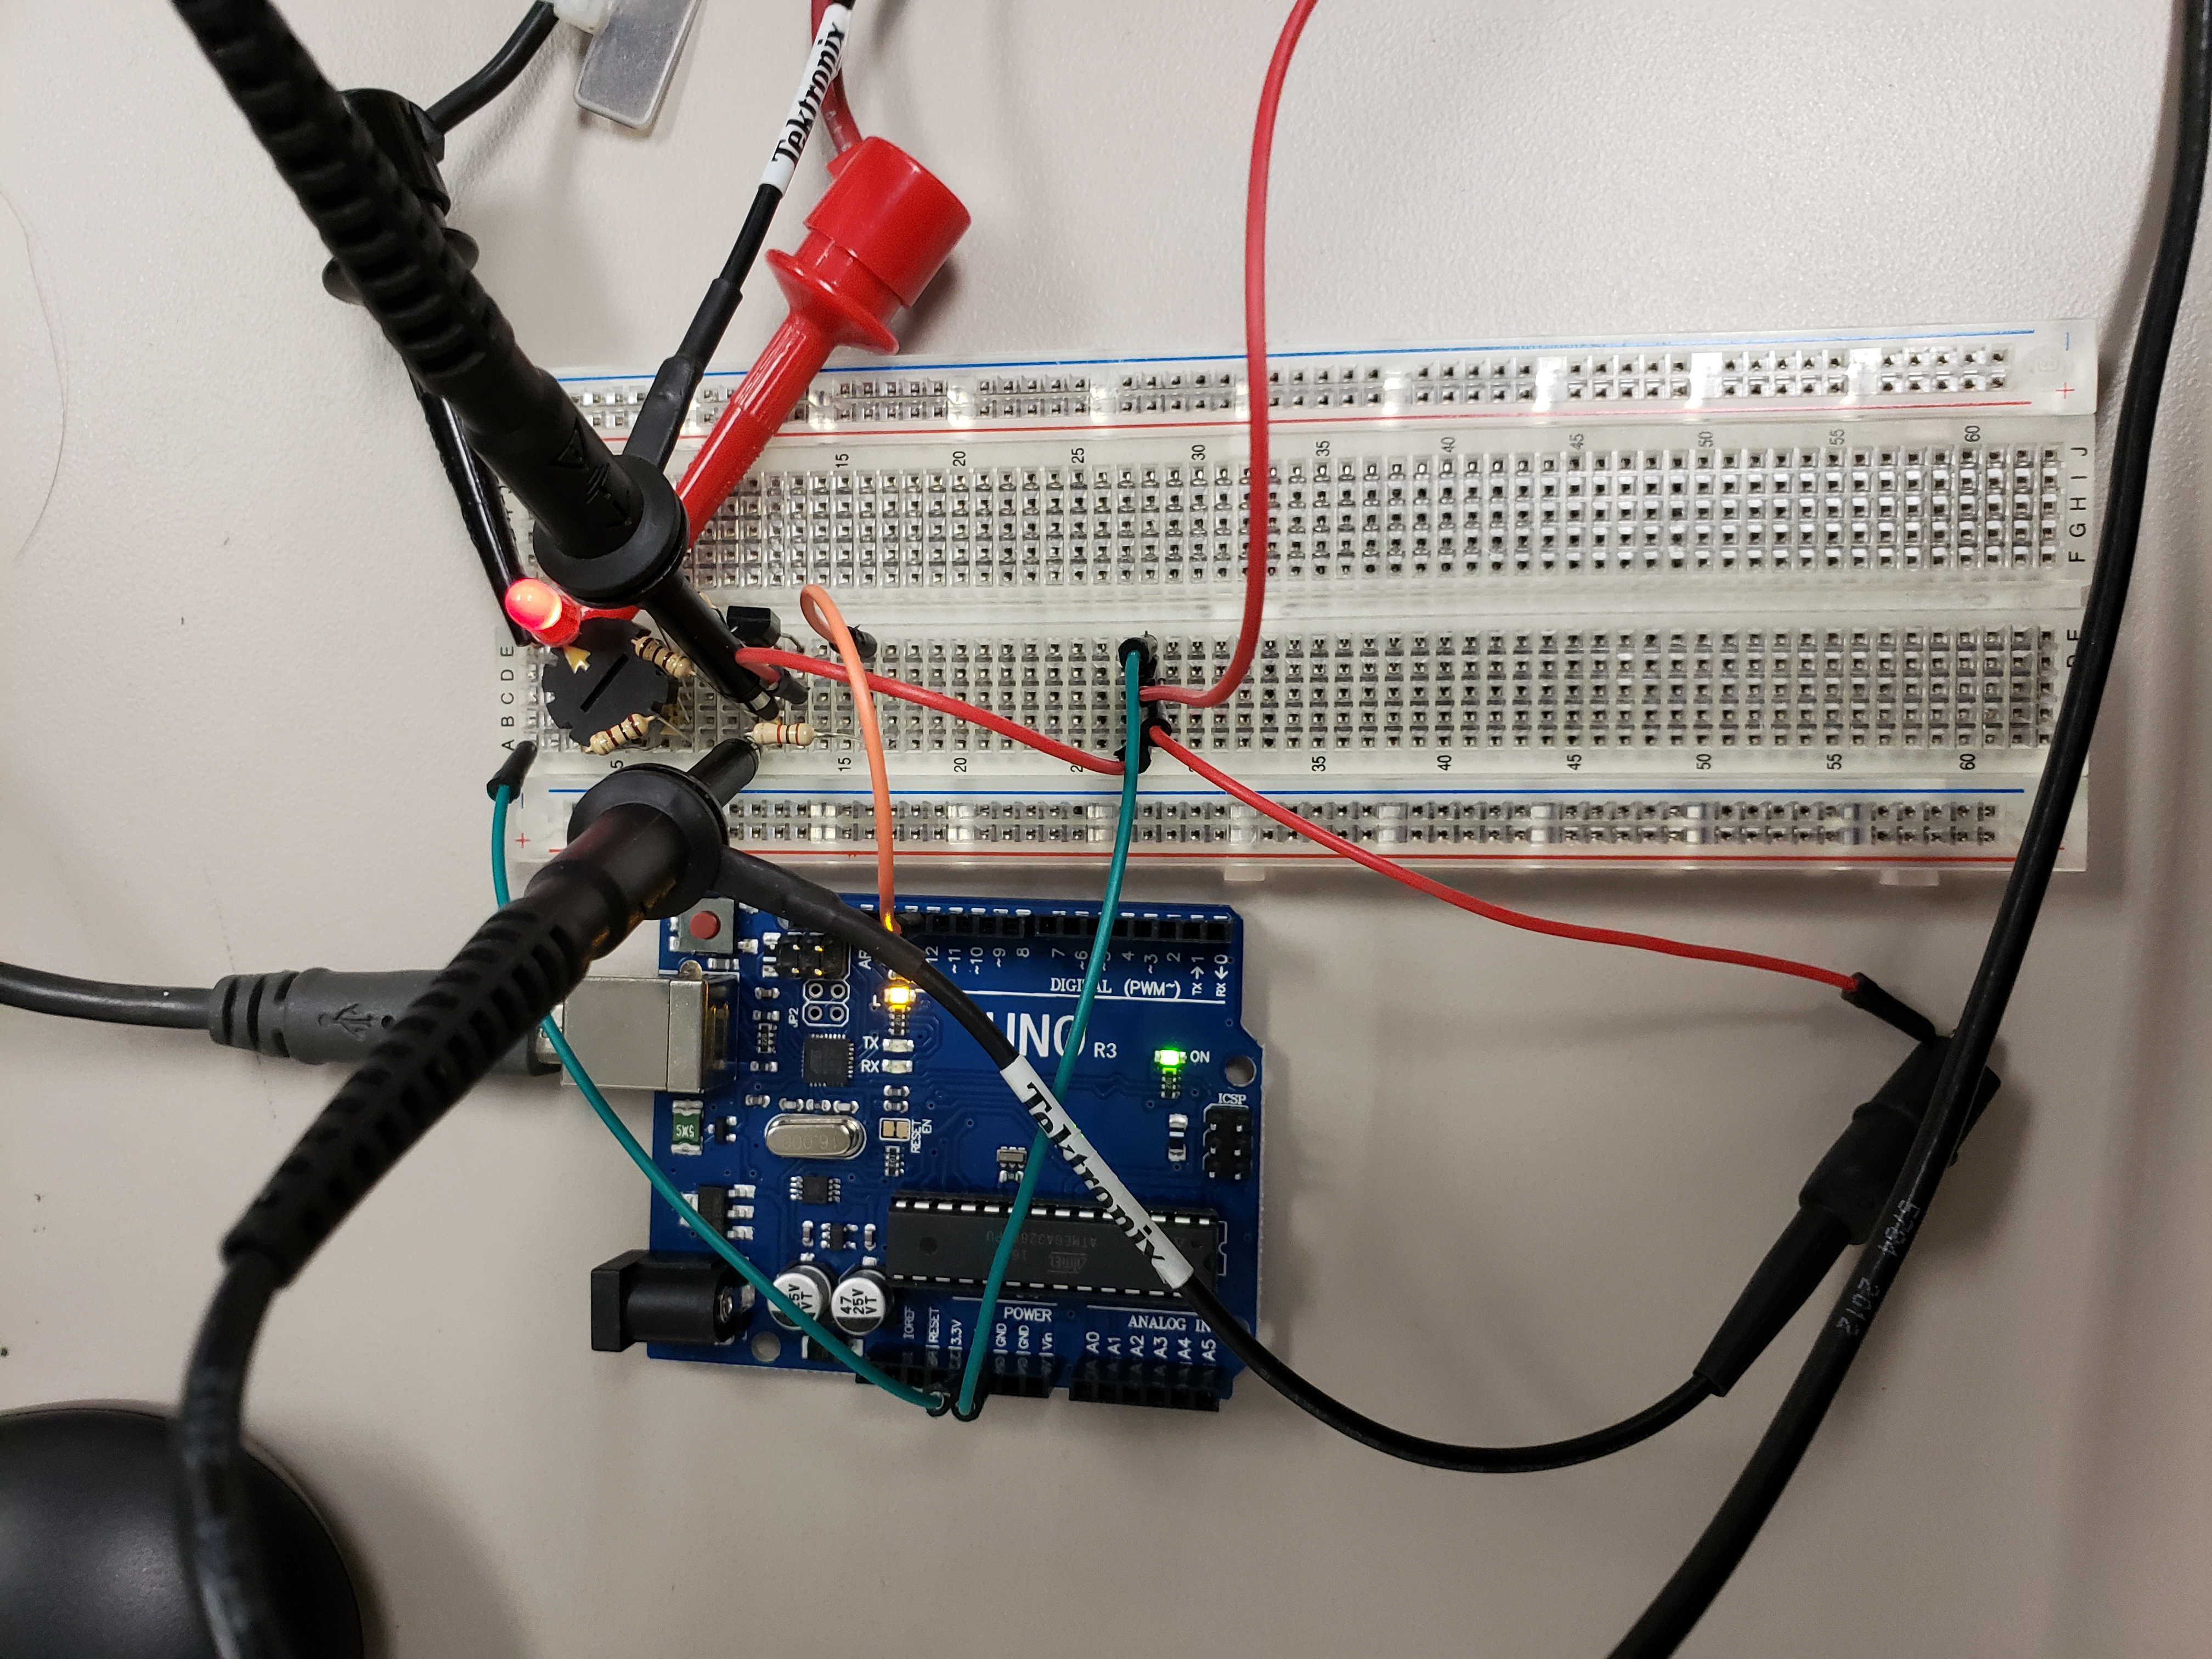
\includegraphics[scale=0.05]{potentiometer.jpg}\\
				\end{center}

				\begin{center}
					\begin{tabular}{|c | c |}
						\hline
						Pot Resistance (Ohms) & LED Current (mA)\\
						\hline
						100 & 6.32 \\
						200 & 7.01 \\
						300 & 7.87 \\
						400 & 8.98 \\
						500 & 10.45 \\
						600 & 12.5 \\
						700 & 15.56 \\
						800 & 20.66 \\
						900 & 30.78 \\
						1000 & 60.85 \\
						\hline
					\end{tabular}
				\end{center}
			
	\section{Lab 3: Tradeoffs Between Hardware \& Software}
		\subsection{Pre-Lab}
			\paragraph{}
				This arduino program reads in two digital inputs at pins 2 and 3 and applies the two inputs into a 'nor gate' then finally that output
				is pushed to pin 4.  Finally it waits one second before reading in the next two inputs.  If you want to decrease the amount of time
				between polls then all you need to do is reduce the amount of time delayed.

				\begin{center}
					\begin{verbatim}
						/*
 						 * Zachary Davis
 						 */

						//initializing various variables
						int analogPin0 = 0;
						int analogPin1 = 0;
						int difference = 0;

						//initialize output pins
						void setup() {
   							pinMode(4, OUTPUT);
						}

						//Constantly check the two inputs and change output based on which
						//of the inputs is higher.
						void loop() {
			  				//Subtract input 2 from 1. If postive 1 is bigger and 
  							//visa versa.
  							difference = analogRead(A0) - analogRead(A1);

  							//If input one is greater set the output ON.
  							//If input two is greater set the output OFF.
  							//If they are equal leave the output as is.
  							if(difference > 0){
    								digitalWrite(4, HIGH);
  							}
  							else if(difference < 0){
    								digitalWrite(4, LOW);
  							}
  							else{
    								delay(1);
  							}

  							//Wait a fifth of a second and start over.
  							delay(200);
						}
					\end{verbatim}
				\end{center}

		\subsection{Boolean Operators in Hardware \& Software}
			\subsubsection{A}
				\paragraph{}
					To complete this portion I build the circuit show below with the addition of an output led to determine more easily
					when the gate outputs high or low.  Below that is the physical circuit after i completed building it.

					\begin{center}
						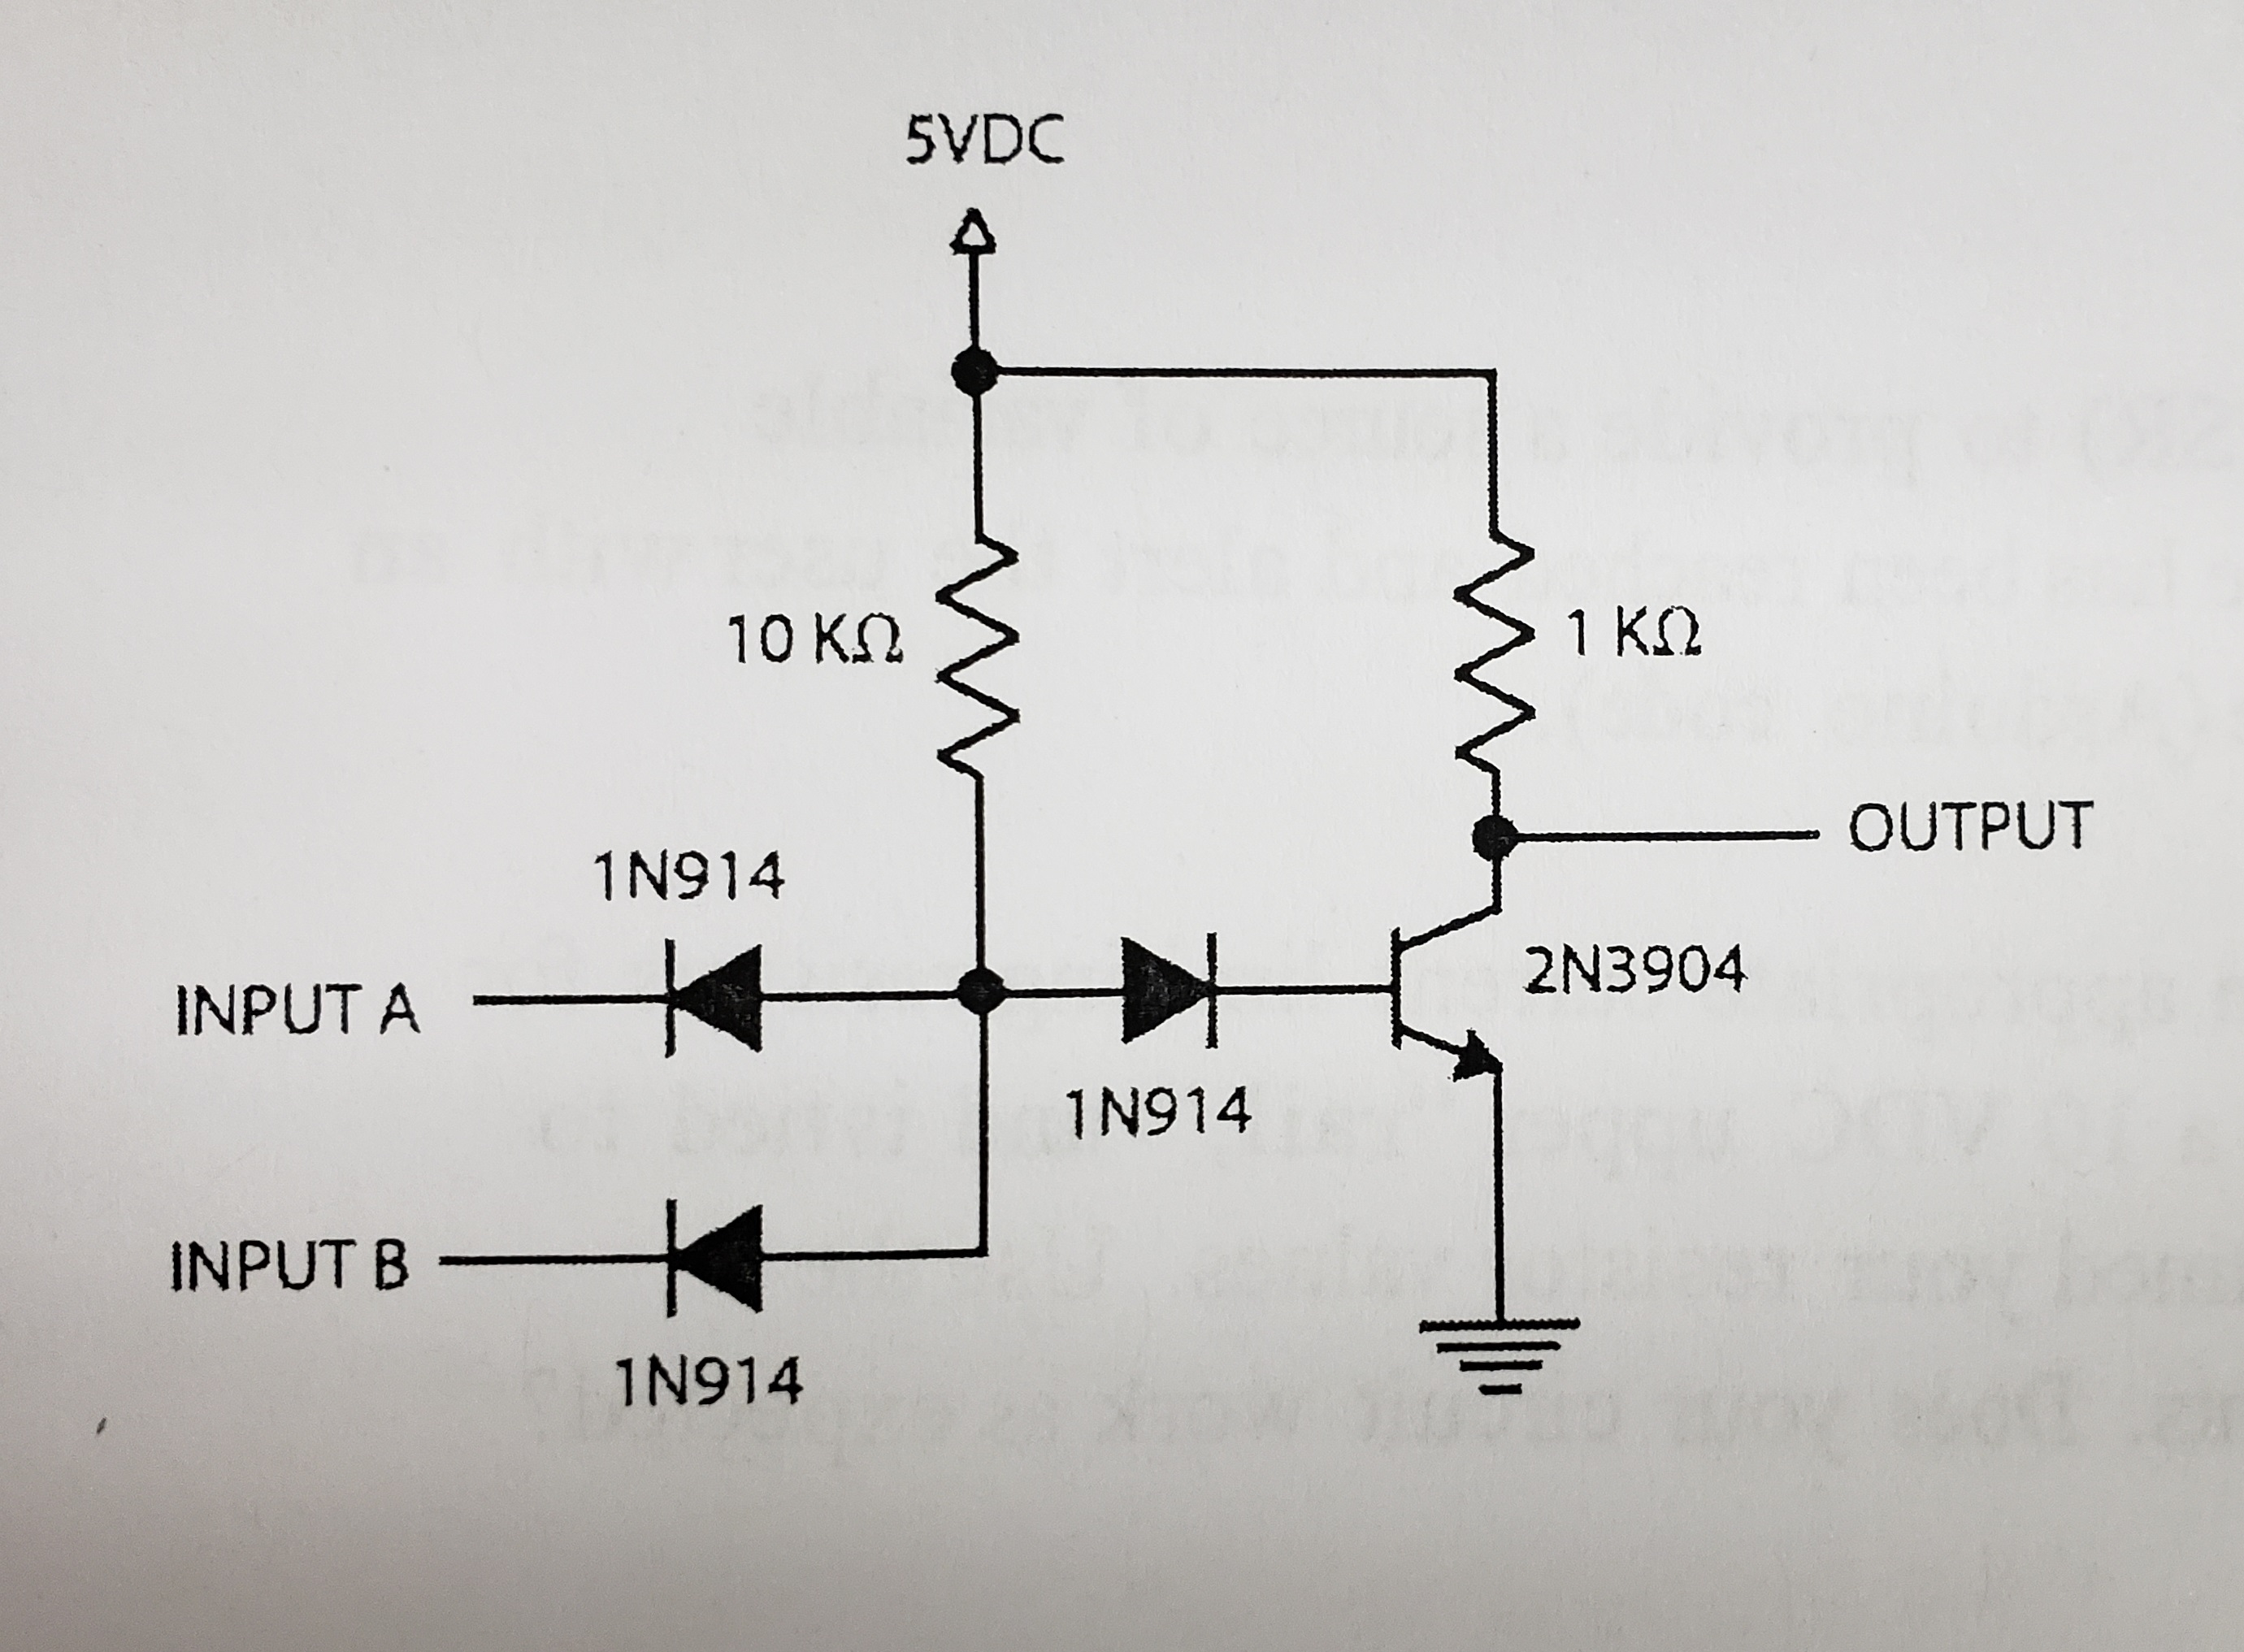
\includegraphics[scale=0.05]{2.jpg}\\
						\vspace{1cm}
						\includegraphics[scale=0.05]{nand.jpg}\\
					\end{center}
			
			\subsubsection{B}
				\paragraph{}
					Having tested all the input cases i have completed the given table...
				
					\begin{center}
						\begin{tabular}{| c | c | c |}
							\hline
							Input A & Input B & Output\\
							\hline
							0 & 0 & 1\\
							0 & 1 & 1\\
							1 & 0 & 1\\
							1 & 1 & 0\\
							\hline
						\end{tabular}
					\end{center}
				
					This is the truth table of a nand gate or inverted and gate.

			\subsubsection{C}
				\paragraph{}
					Completing the simple circuit below with the 7400 integrated circuit i found that this was i prebuilt nand gate and therefore
					exactly the same as the more complicated circuit from the previous part.
					
					\begin{center}
						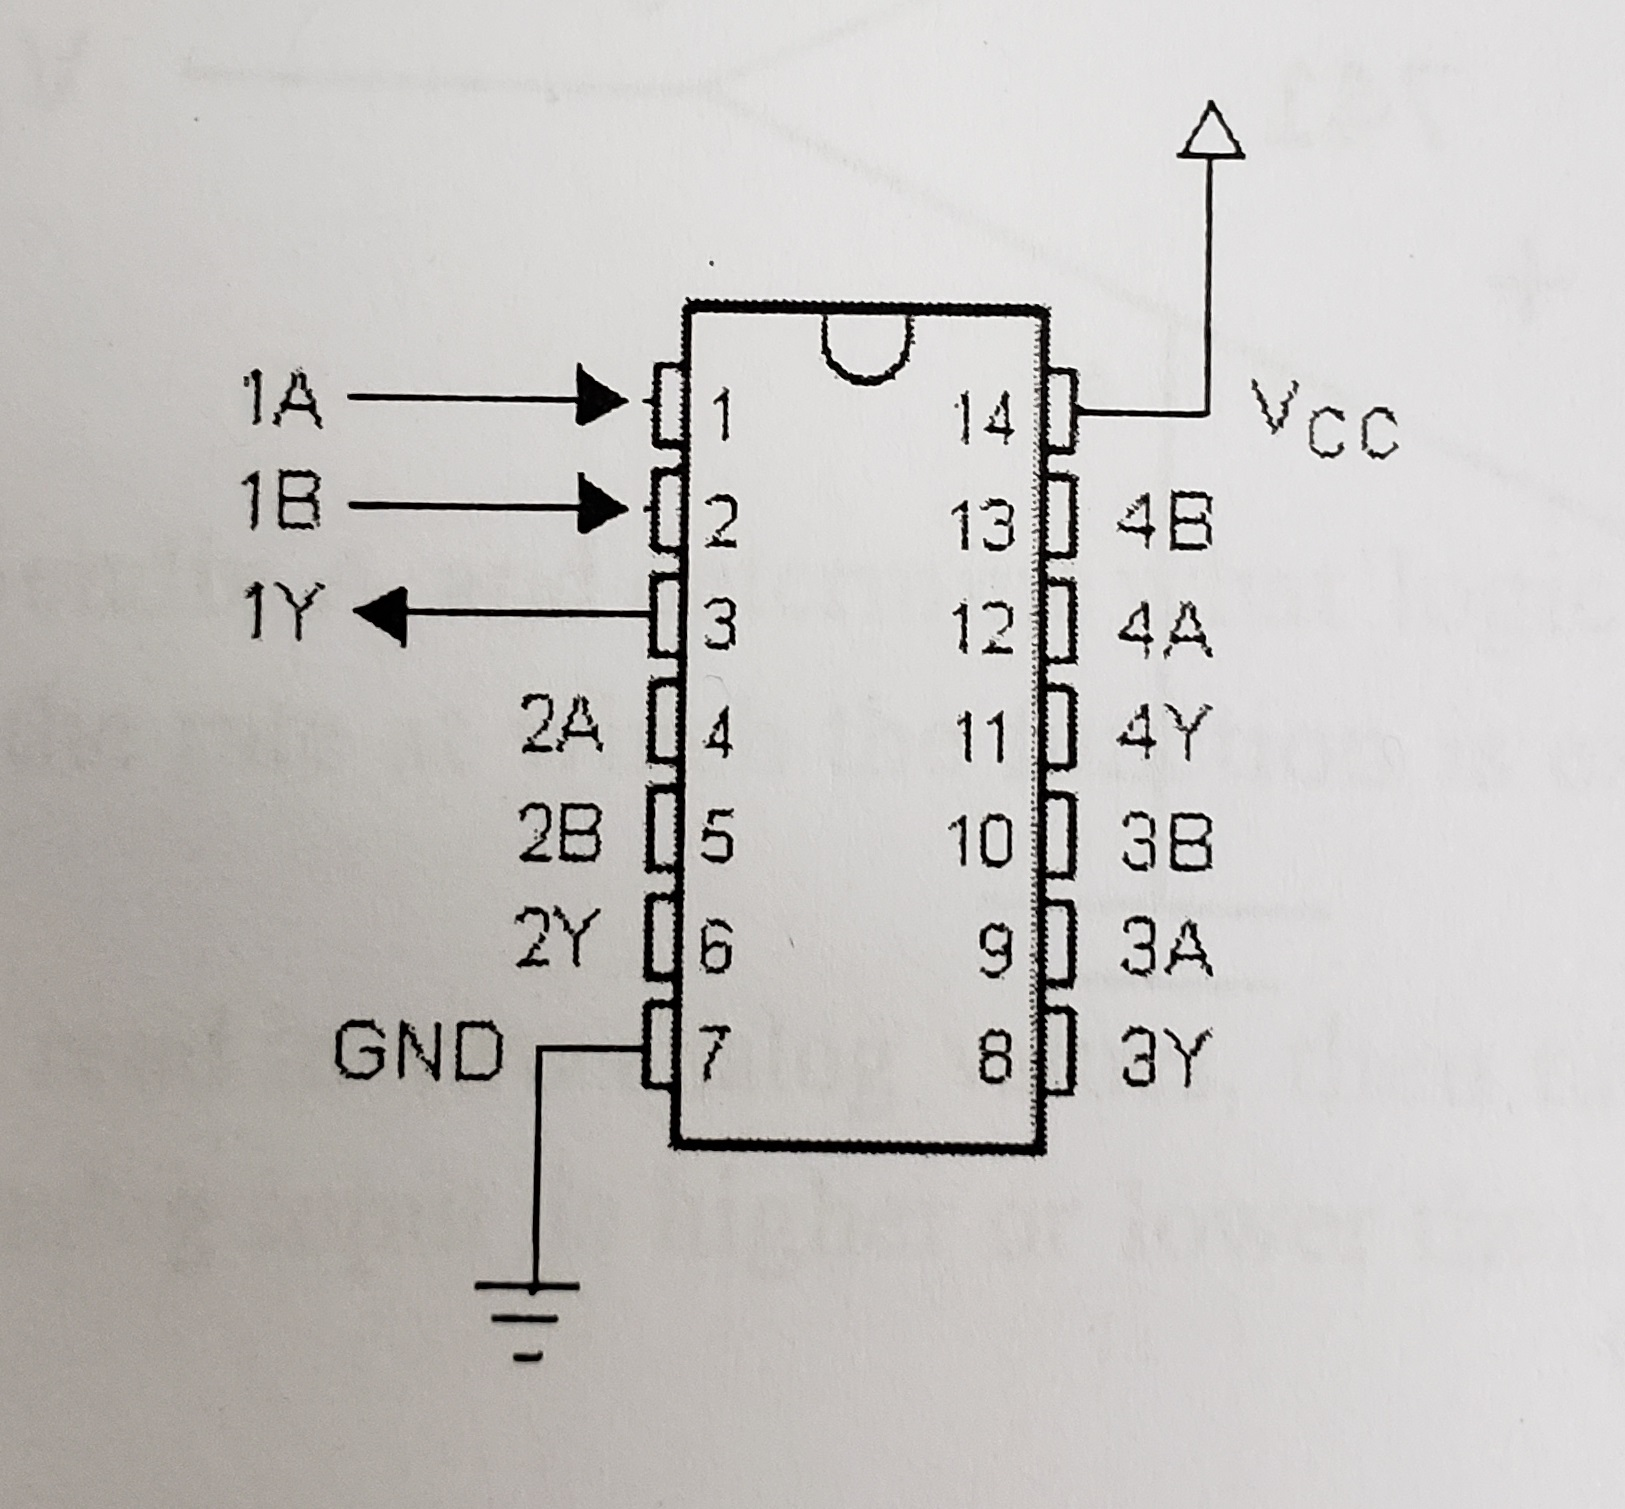
\includegraphics[scale=0.08]{mystery.jpg}\\
					\end{center}

			\subsubsection{D}
				\paragraph{}
					For this portion of the lab I applied a square wave of amplitude 2.5V to both inputs simutaneously and viewed the input and output of the circuits
					logic on the oscope, which you can see below.  You can already see there is and every so slight delay between the two but then when i ploted an
					equation showing the delay as a function you can see the exact impact.

					\begin{center}
						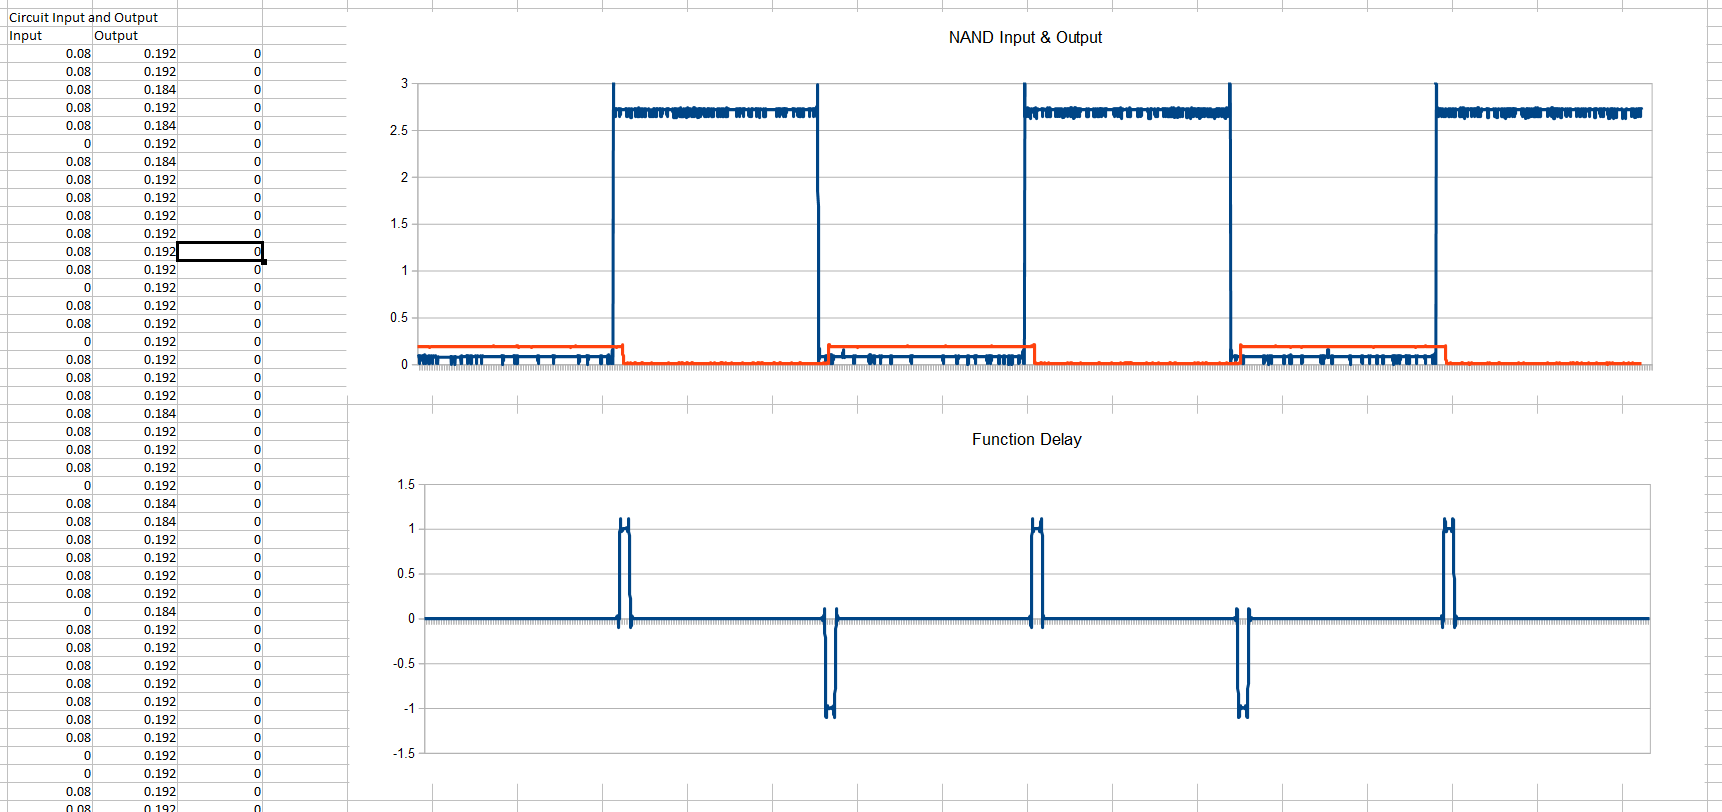
\includegraphics[scale=0.2]{delay.png}\\
					\end{center}

			\subsubsection{E}
				\paragraph{}
					In this part of the lab I wrote an arduino program that acted as a NAND gate with inputs at pins 2 and 3 and output at pin 4.  For more detail read the 
					comments in the code.

					\begin{center}
						\begin{verbatim}
							/*
							 * Zachary Davis
							 */

							//initializing various variables	
							int digitalPin0 = 0;
							int digitalPin1 = 0;

							//initialize output pins
							void setup() {
  					 			pinMode(4, OUTPUT);
							}

							//Constantly check the two inputs and change output based on which
							//the truth table of a NAND gate.
							void loop(){
								//Read in from both input pins and AND them then NOT them in that results in a 1 the if is grabbed
  								if(!(digitalRead(2) && digitalRead(3))){
    									digitalWrite(4, HIGH);
  								}
								//Otherwise write to low
  								else{
    									digitalWrite(4, LOW);
  								}
							}
						\end{verbatim}
					\end{center}

			\subsubsection{F}
				\paragraph{}
					When repeating step D on the arduino code to see the delay the results are better there did not appear to be any noticable delay and once
					i applied and equation to plot the delay and again you can see that there is none.  Note that the reason they are all perfectly zero is because
					if the resulting data point was below a 0.10 threshold it was rounded down to zero to make the graph more clear that there was no delay.

					\begin{center}
						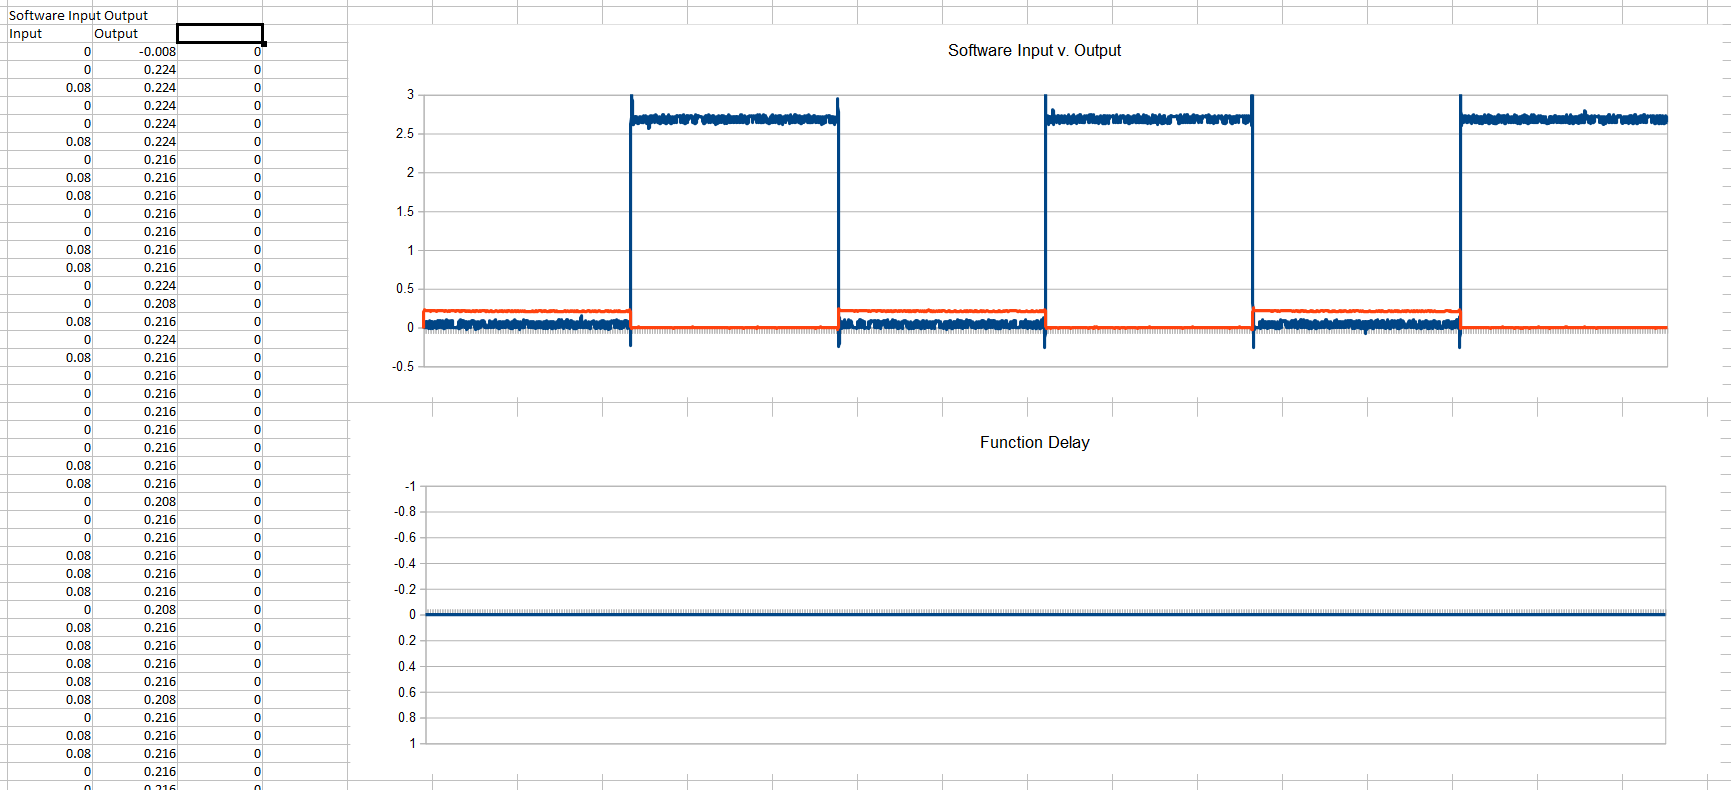
\includegraphics[scale=0.2]{nodelay.png}\\
					\end{center}
			
			\subsubsection{G}
				\paragraph{}
					When you are creating logic gates with circuits there are two very clear benefits.  Because you are building the gates on a circuit level everything
					can be more clearly diagnosed and can be followed on the lowest level which is helpful in specific use cases.  Another is the low cost of and 
					temperary nature of the circuit.  If you are building and integrated circuit like a seatbelt sign on a plane it is far cheaper and easier to prototype 
					with a circuit that to buy a microcontroller just to have a smaller dedicated IC fabricated once you are done.  However, these circuits are big and 
					bulky and if you want to make any minor behavioral adjustments it is very time consuming and more prone to mistakes.

			\subsubsection{H}
				\paragraph{}
					A clear benefit to using software and a microcontroller to develop logic circuits is the lack of a need of physical reasources.  Beyond the microcontroller
					and its RAM limites you can build far more large and complex circuits without needed more and more elements like with a circuit.  Another advantage of 
					using a microcontroller is the space savings when the complexities of your circuits is scaled up, which is of course why embedded systems are custom
					fabricated ICs from a software schematic.  You do not have the same granular control that you do with a circuit and the diagnosis of problems can be
					more difficult, not to mention that when you want to have it fabricated to an IC you have to design that as well.

		\subsection{Force Sensistive Alarm in Hardware \& Software}
			\subsubsection{A}
				\paragraph{}
					Below you can see the circuit I was supposed to build and the corresponding physical circuit.  For the current limiting resistors i used 150 Ohms
					for the led and 1 kOhms for the b pin on the transistor from the experiences earlier in this lab.  The circuit works exactly as expected.  You use the 
					potentiometer to select the threshold and once that is reached with the FSR then the led will illuminate all be in rather dim.  

					\begin{center}
						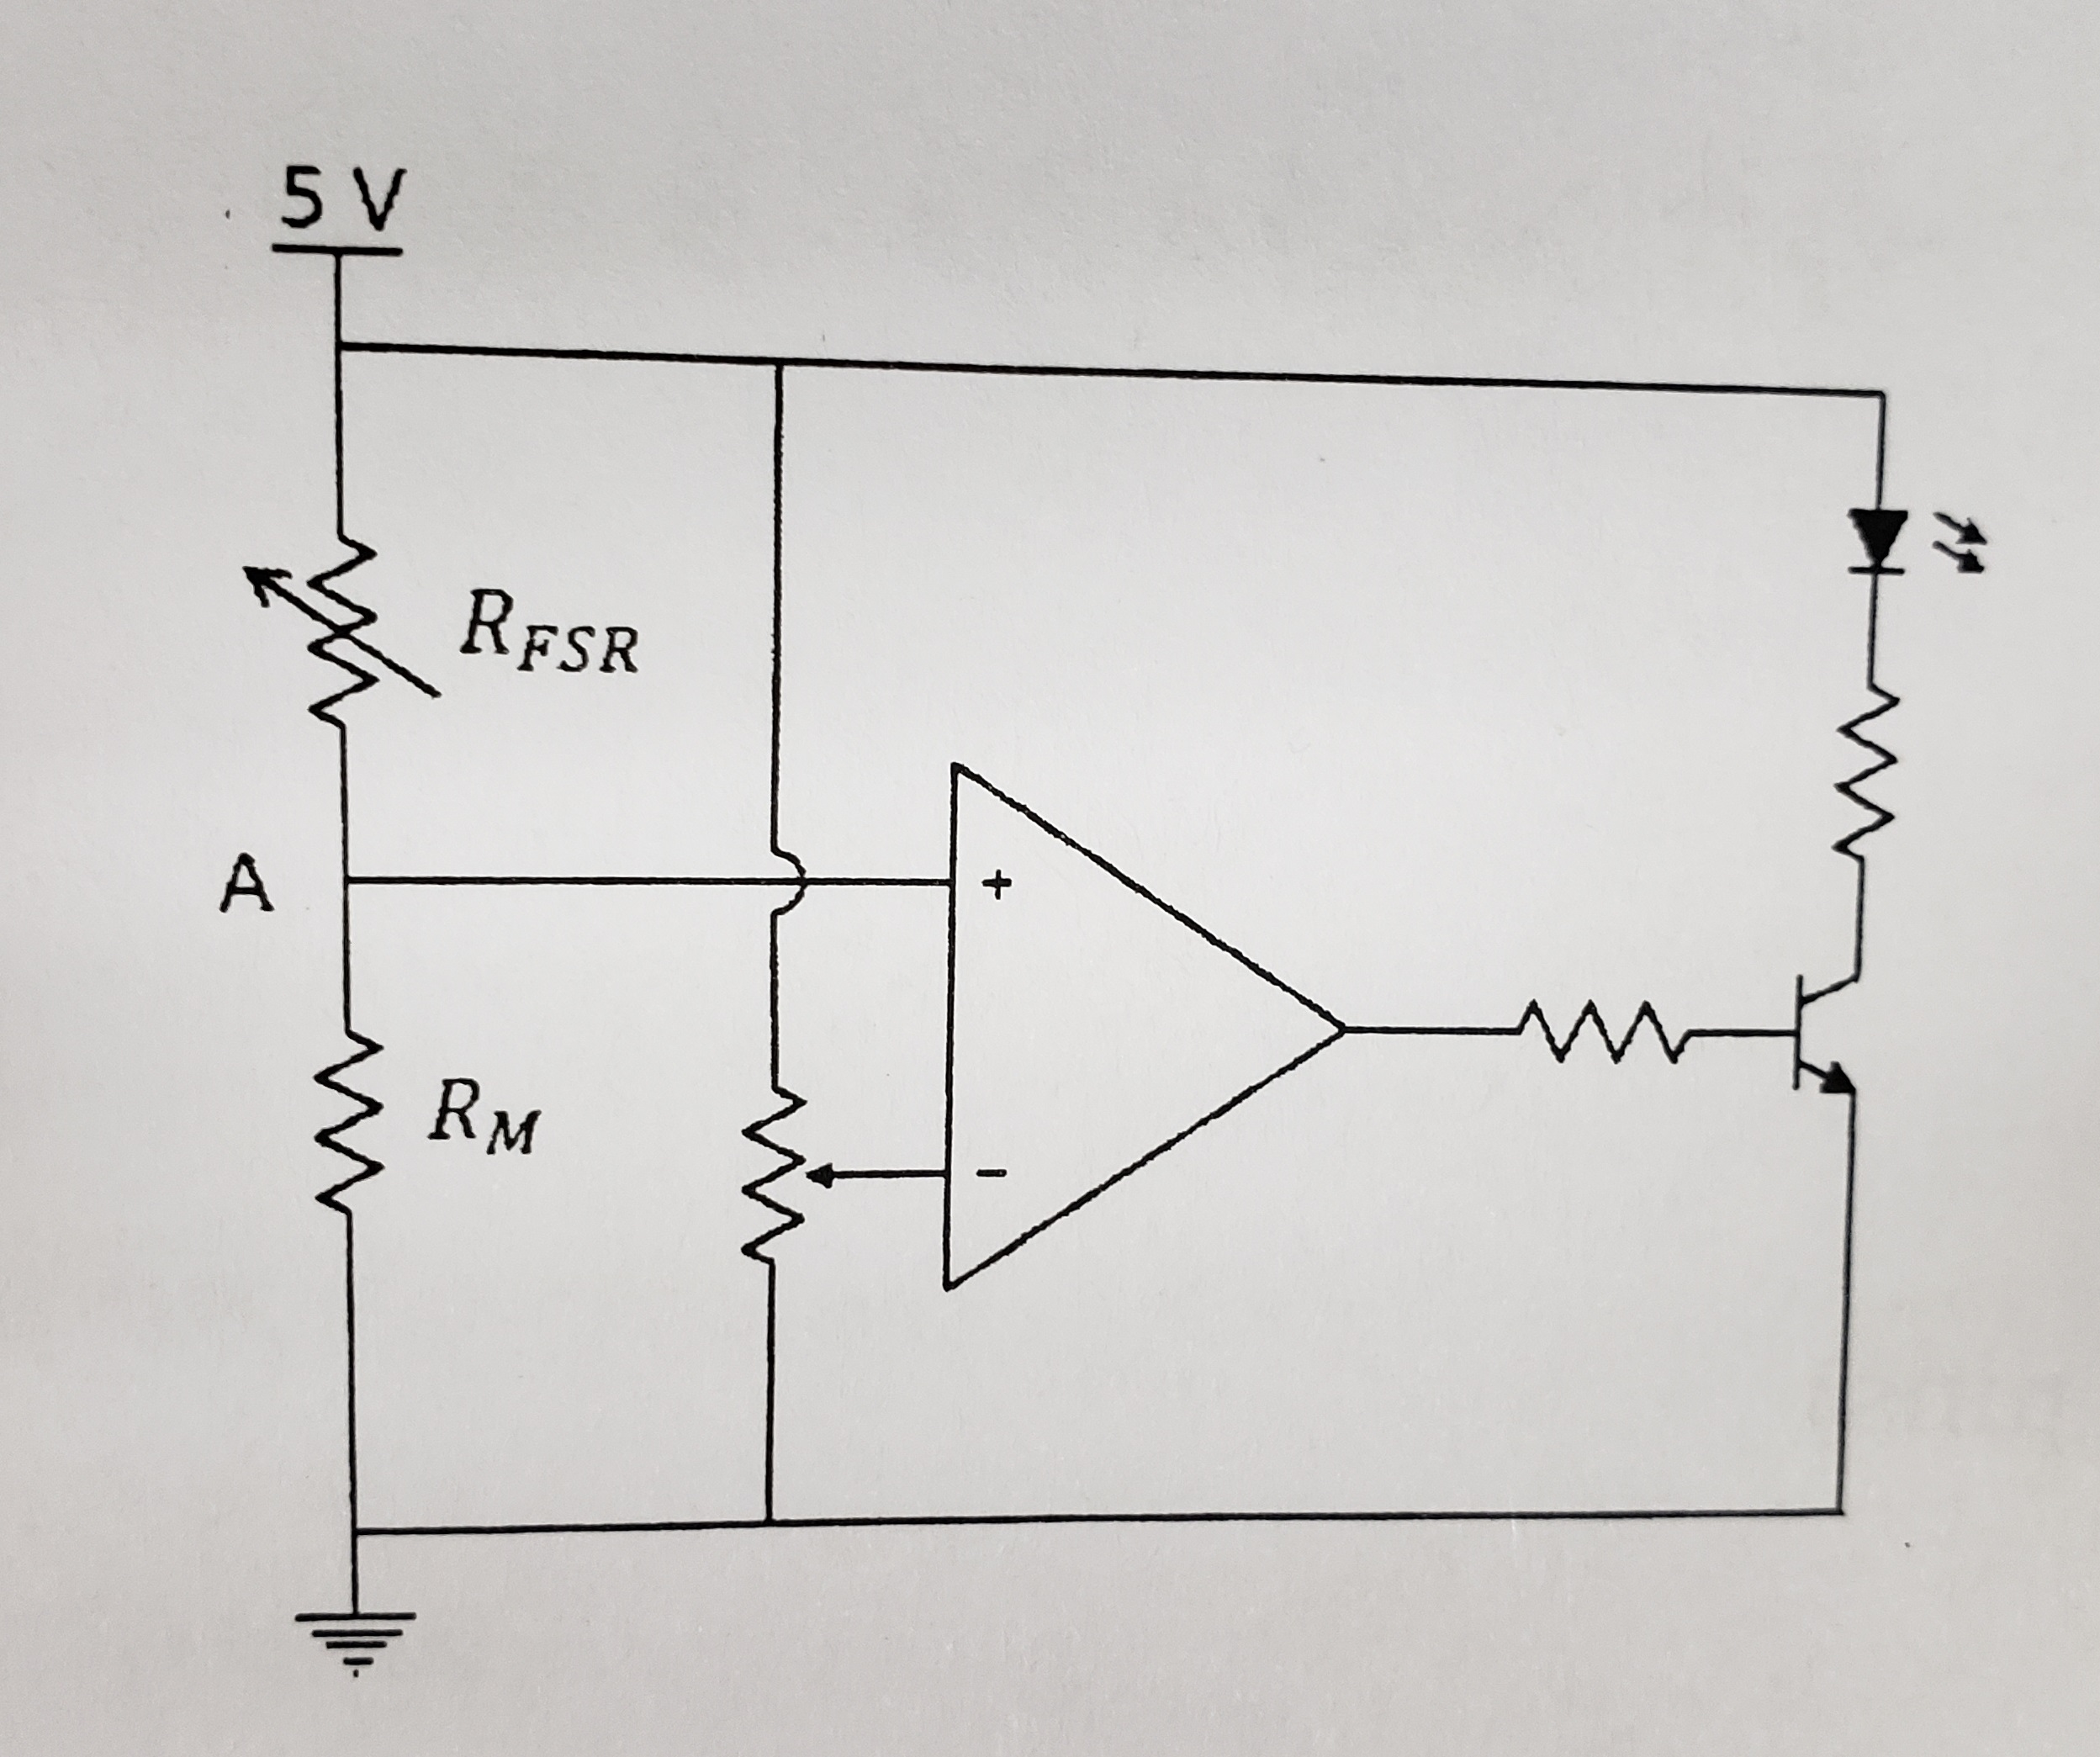
\includegraphics[scale=0.05]{3.jpg}\\
						\vspace{1cm}
						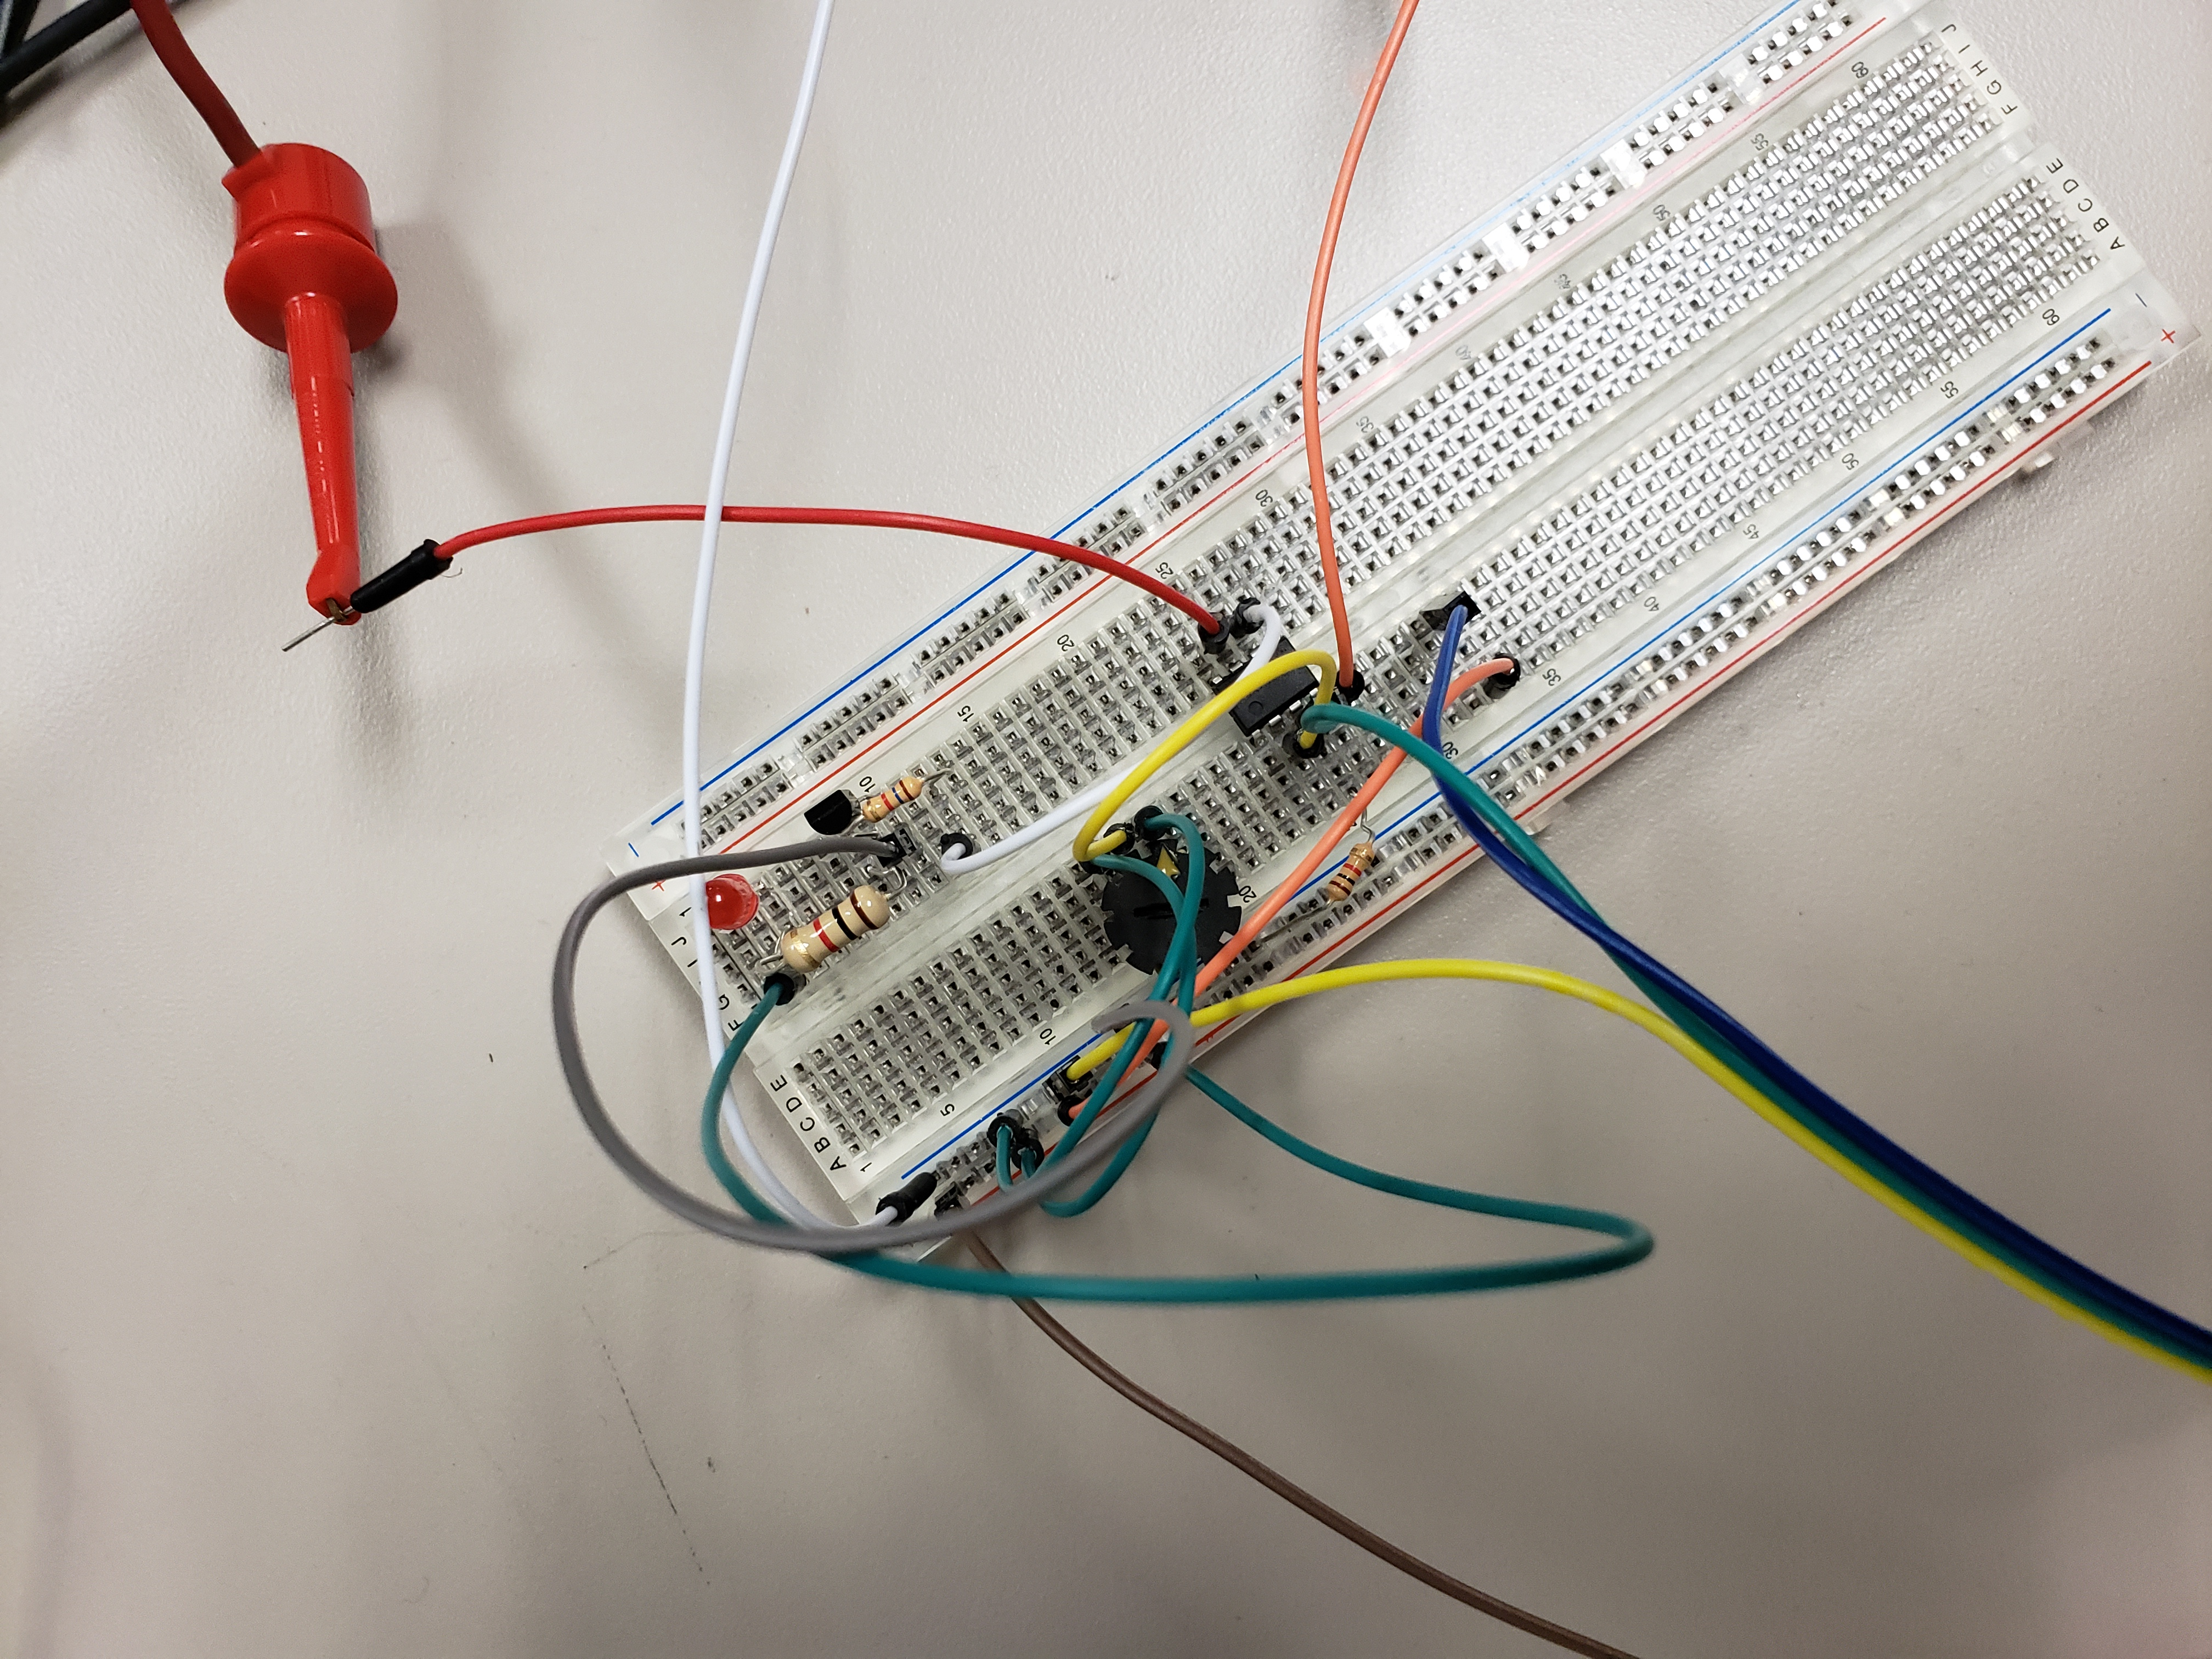
\includegraphics[scale=0.04]{fsr.jpg}\\
					\end{center}
			
			\subsubsection{B}
				\paragraph{}
					If i was to implement this on the arduino it would start of very similar to the code from the pre-lab.  I would intake the voltage drop in a very simple circuit 
					where the FSR is connected in series with another resister and power.  That in turn would correlate to the applied force.  Finally that would be compared
					to a hard coded constant in an if else bracket which would determine the light status of the on board led to show if the threshold has been surpassed.

			\subsubsection{C}
				\paragraph{}
					These really are the same as the were for the advantages and disadvantages listed above from the logic gate portion of the lab.

			\subsubsection{D}
				These really are the same as the were for the advantages and disadvantages listed above from the logic gate portion of the lab.

	\section{Lab 4: Analog Input \& Output}
		\subsection{Pre-Lab}
			\subsubsection{1}
				\paragraph{}
					analogRead() is a function in arduino's ide that will read in an analog value from 0 to 5 volts and use a A2D converter to remap that to 0 to 1023 bits
					to represent the value digitally.

			\subsubsection{3}
				\paragraph{}
					analogWrite() will output a value from 0 to 255 to a specified pin. The number represents the duty cycle of the square wave from 0 always of to 255 always
					on giving you 8 bits or 1 byte of granularity.

			\subsubsection{4}
				\paragraph{}
					PWM pins need to be specified as outputs in te setup function but not in a more special way then any other output pin.

			\subsubsection{5}
				\paragraph{}
					The duty cycle of analongWrite(11, 127) is 127 to pin 11.  A more useful way to look at that is 127/255*100 percent of the time on and 
					the rest of the time off.

			\subsubsection{6}
				\paragraph{}
					For this portion of the lab i was to write an arduino program that reads in an analog value prints that to the serial monitor and remaps that to output 
					the same voltage as pwm.  Below is my code.

					\begin{center}
						\begin{verbatim}
							/*
							 * Zachary Davis
							 */

							//initializing various variables
							int analogIn = 0;
							int analogOut = 0;

							//initialize output pins
							void setup(){
  				 				pinMode(3, OUTPUT);
							}

							void loop(){
  								//Read the analog value in from A0
  								analogIn = analogRead(A0);
  								//Print this value to the monitor
  								Serial.println(analogIn);
  								//Use the equation to remap to PWM range keeping ratio equal
  								analogOut = (analogIn/1023)*255;
  								//Write this value to out PWM pin 3
  								analogWrite(3, analogOut);
							}
						\end{verbatim}
					\end{center}

		\subsection{Analong Input \& Output}
			\subsubsection{A}
				\paragraph{}
					To start this lab we were instructed to build the below circuit...
					
					\begin{center}
						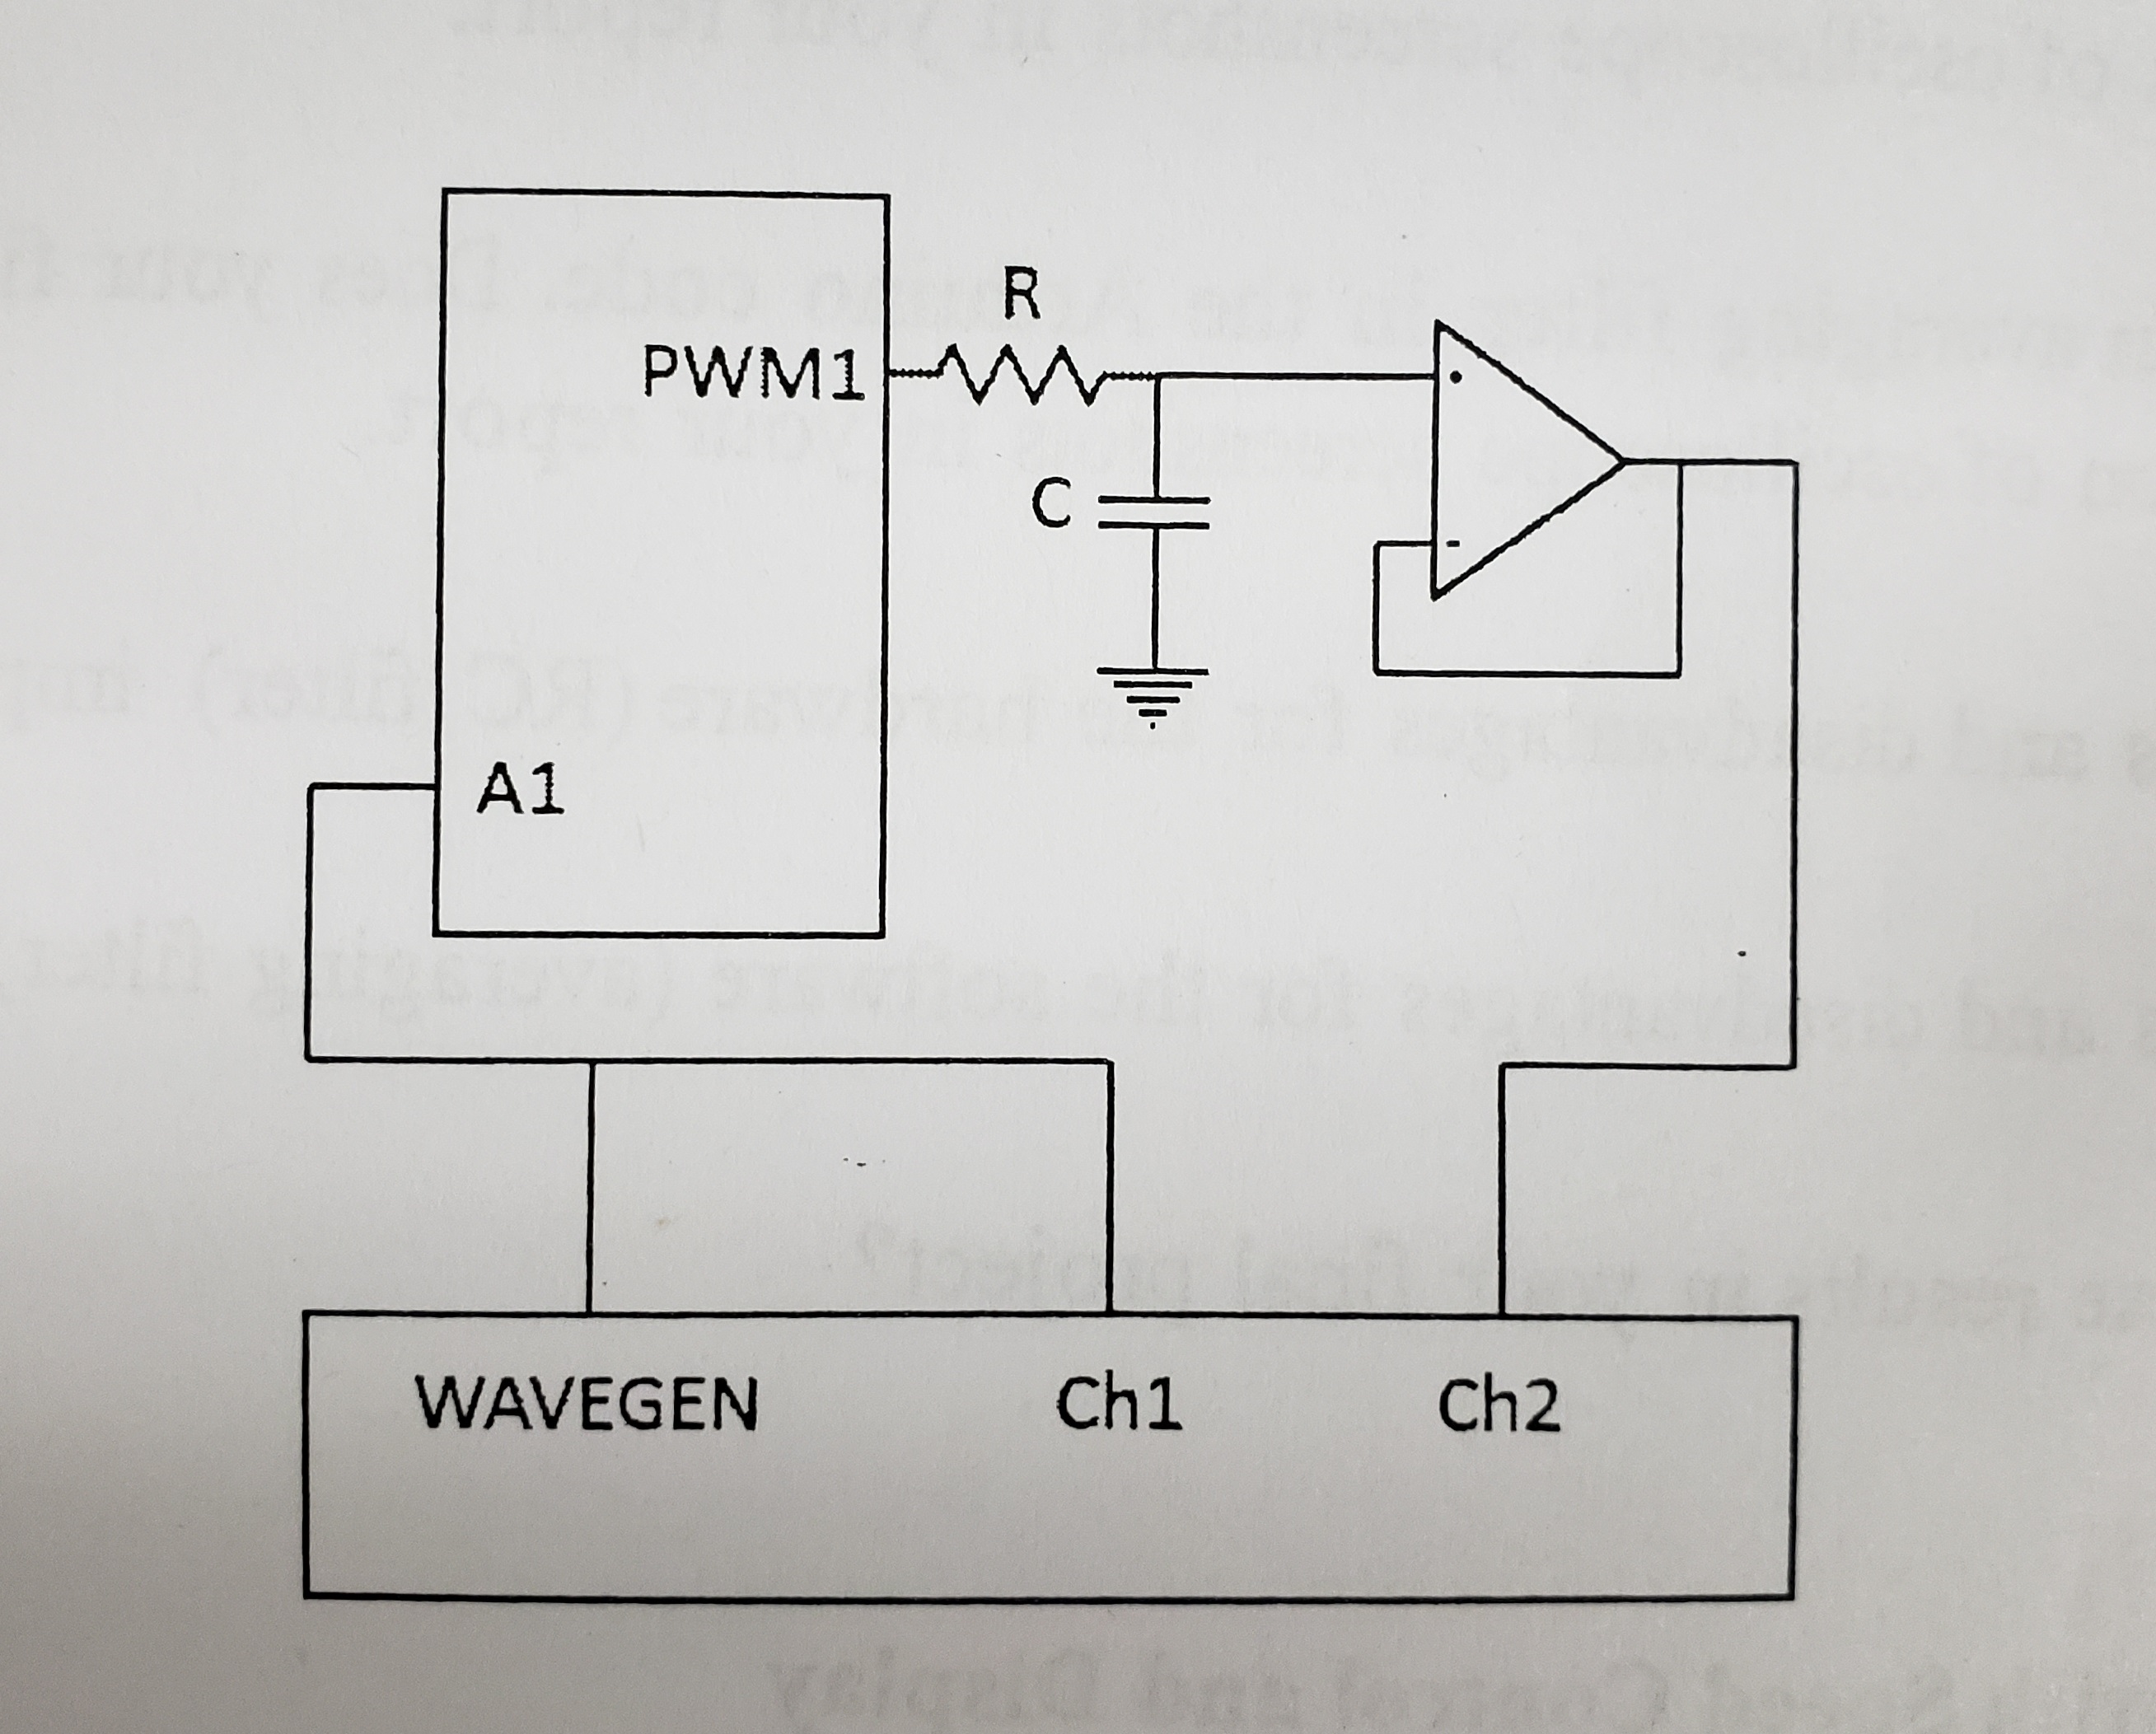
\includegraphics[scale=0.04]{4.jpg}\\
					\end{center}

					We choose R to be 16 kOhms and C to be 0.1 uF giving a frequency cutoff of 100 Hz.  Then we loaded the pre-lab code shown above
					onto the arduino.  Below is the physical circuit itself.
					
					\begin{center}
						\includegraphics[scale=0.04]{analog.jpg}\\
					\end{center}
			
			\subsubsection{B}
				\paragraph{}
					Once the circuit was complete we applied a 0 to 5V 10 Hz input into the arduino and used one channel to monitor the input and another to 
					monitor the output.

			\subsubsection{C}
				\paragraph{}
					The numbers in the serial monitor represent the voltage of the analog signal remapped to 0-1023 from 0-5 keeping an equal ratio of course.

			\subsubsection{D}
				\paragraph{}
					The quantization error is defined as...
						
					\begin{equation}
						SQNR = 20log_{10}(2^Q)
					\end{equation}

					Which in our case as it is a 10 bit A2D comes out to 60.206 dB.

			\subsubsection{E}
				\paragraph{}
					The outputs when you do not print the values to the serial monitor look exactly as you should expect.  The amplitude is as close as makes no
					difference.  The period is the same, the only difference is the analog sine wave is essentially converted to a PWM or square wave.  When you 
					first print to the serial monitor your output wave is ever so slightly out of phase which gets worse and worse the higher the input frequency.  This 
					is because it is a serial monitor and acts serially.  The arduino firsts communicated to the computer then the output is pushed causing the delay.  
					You can see both cases below.

					\begin{center}
						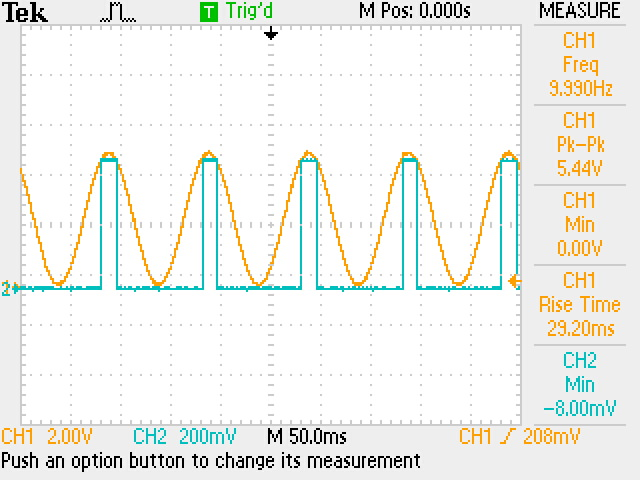
\includegraphics[scale=0.5]{noserial.jpg}\\
						\vspace{1cm}
						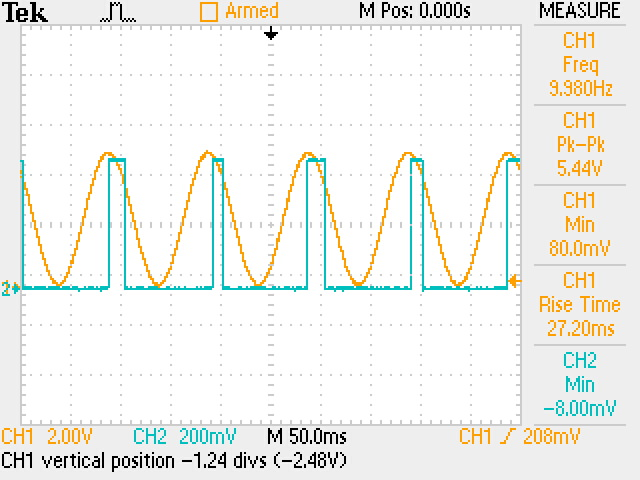
\includegraphics[scale=0.5]{serial.jpg}\\
					\end{center}

			\subsubsection{F}
				\paragraph{}
					The input and output no longer match when the output frequncy goes beyond that of he low pass filter.  When the input starts to get larger than 100
					Hz in my case the output is then filtered out as that is the job of the low pass.  This can be seen below when we go way beyond 100 Hz.

					\begin{center}
						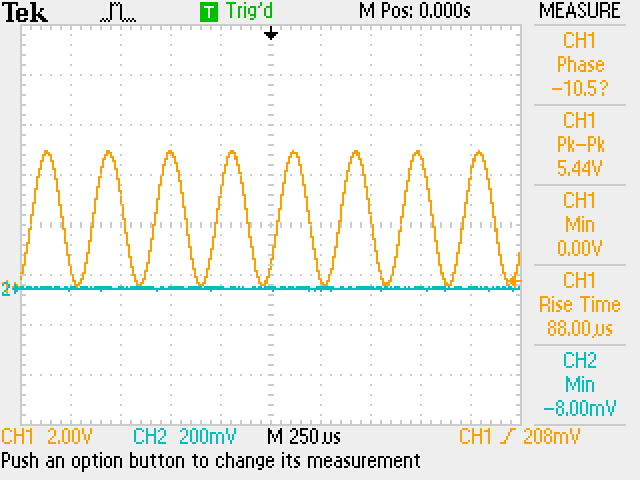
\includegraphics[scale=0.5]{gone.jpg}\\
					\end{center}

		\subsection{Analong Sensor Reading}
			\subsubsection{A}
				\paragraph{}
					The function generator is replaced with the ir sensor as shown below.

					\begin{center}
						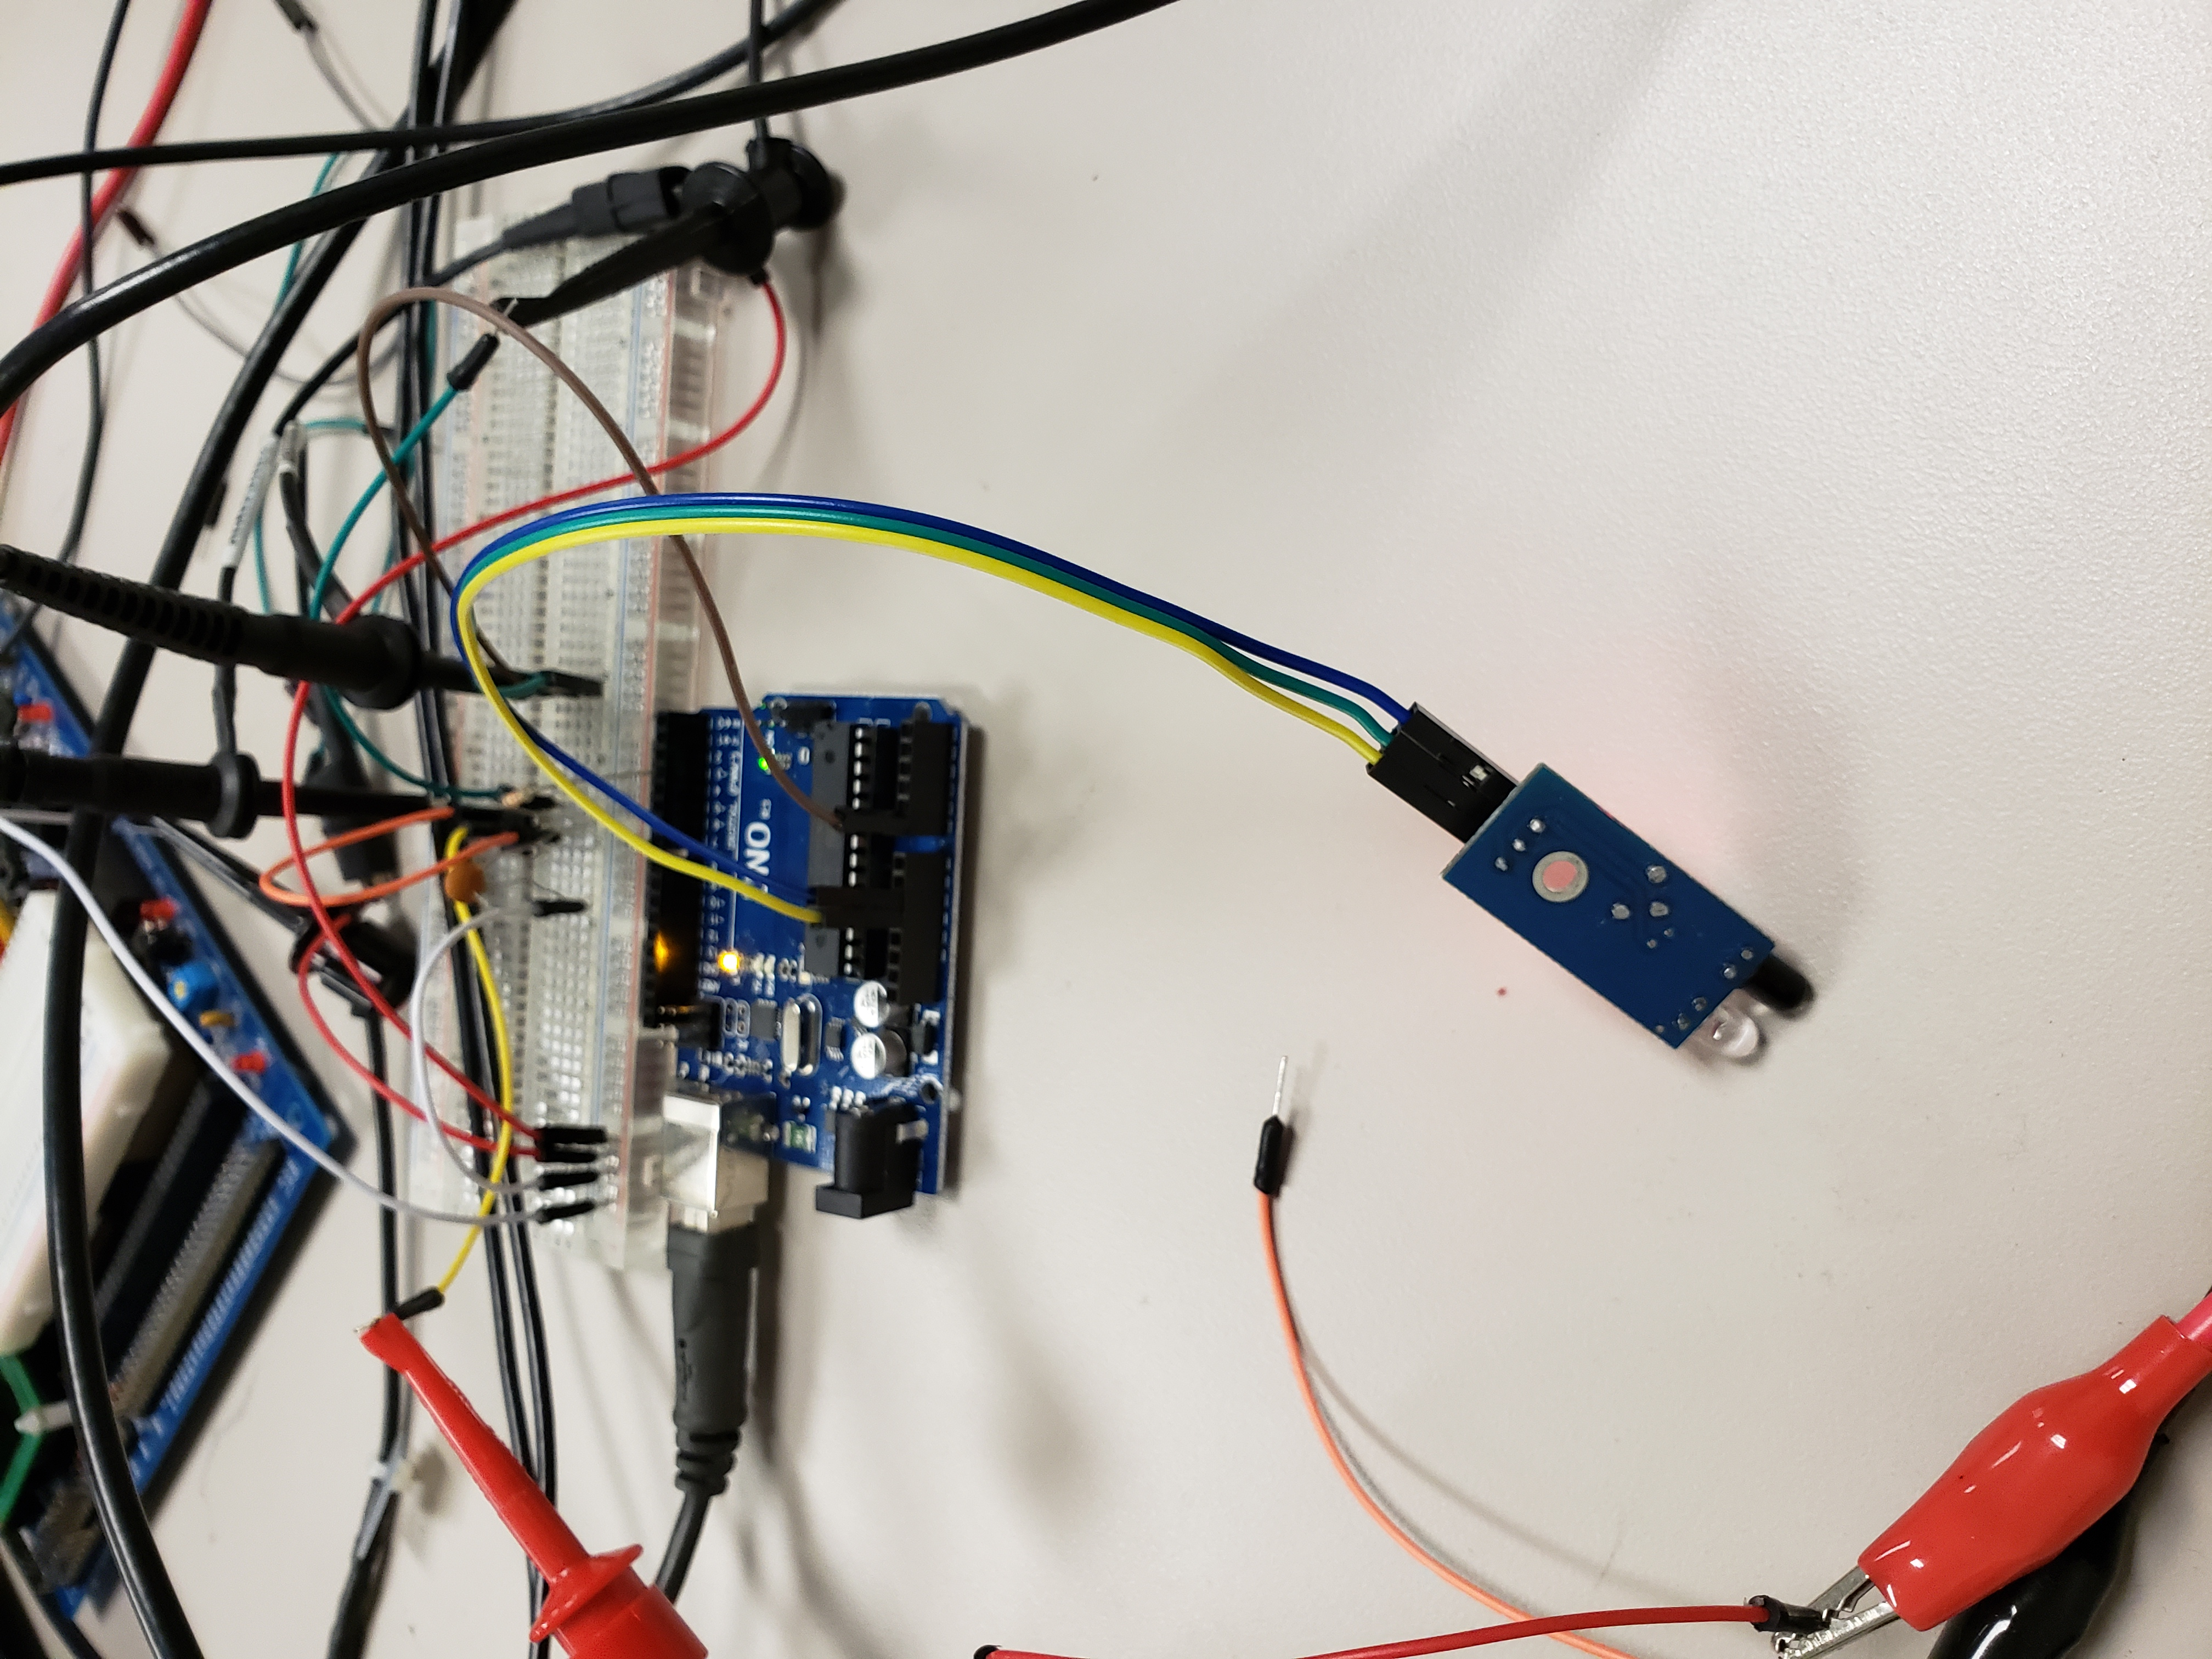
\includegraphics[scale=0.05]{ir.jpg}\\
					\end{center}
			
			\subsubsection{B}
				\paragraph{}
					The average voltage of the noise of the IR sensor is about 1.48 volts and has a pk-pk voltage of anywhere from 300-800 mV.  The oscope wave
					form is shown below

					\begin{center}
						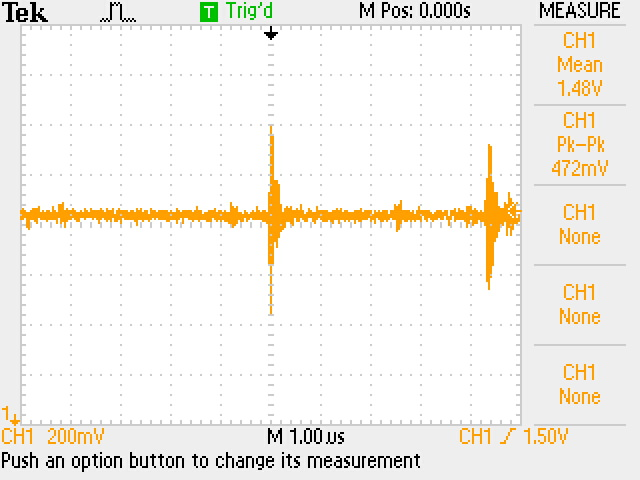
\includegraphics[scale=0.5]{irnoise.jpg}\\
					\end{center}

			\subsubsection{C}
				\paragraph{}
					At the abosolute most the IR sensor will go as low as 280 mV or as high as 1.88 volts meaning that the range of inputs should be around 57-385
					and i never saw a number outside of that range go by on the serial monitor.

			\subsubsection{D}
				\paragraph{}
					The maximum amplitude of the noise spike is around 1.78V and a screenshot has been included below.

					\begin{center}
						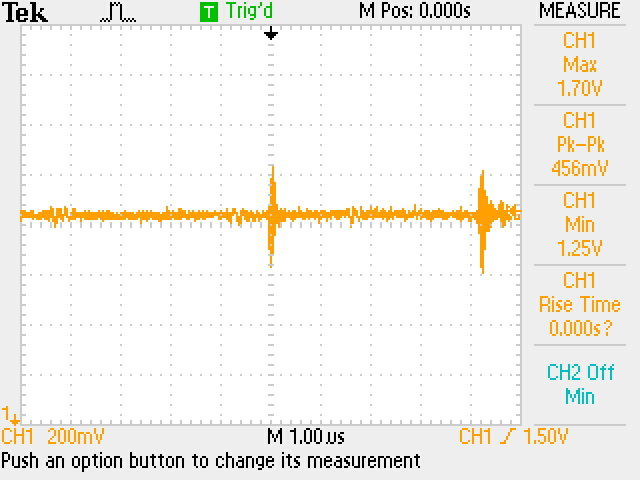
\includegraphics[scale=0.5]{spike.jpg}\\
					\end{center}

			\subsubsection{E}
				\paragraph{}
					My previous calculation of range spanned included the noise spike so the range remains at 57-385.

			\paragraph{}
				I did not have time to complete the remaining portion of this lab or attempt the bonus segment of this lab, however i have included previously 
				written code i wrote to create a seven segement display at least as proof of understanding.

				\begin{verbatim}
					module Seven_Segment_Display(In3, In2, In1, In0, A, B, C, D, E, F, G);
input In3, In2, In1, In0;
output A, B, C, D, E, F, G;
reg A, B, C, D, E, F, G;
always@*
begin
A = (!In3 & !In2 & !In1 & !In0) | (!In3 & !In2 & In1 & !In0)
| (!In3 & !In2 & In1 & In0) | (!In3 & In2 & !In1 & In0)
| (!In3 & In2 & In1 & !In0) | (!In3 & In2 & In1 & In0)
| (In3 & !In2 & !In1 & !In0) | (In3 & !In2 & !In1 & In0)
| (In3 & !In2 & In1 & !In0) | (In3 & In2 & !In1 & !In0)
| (In3 & In2 & In1 & !In0) | (In3 & In2 & In1 & In0);
B = (!In3 & !In2 & !In1 & !In0) | (!In3 & !In2 & !In1 & In0)
| (!In3 & !In2 & In1 & !In0) | (!In3 & !In2 & In1 & In0)
| (!In3 & In2 & !In1 & !In0) | (!In3 & In2 & In1 & In0)
| (In3 & !In2 & !In1 & !In0) | (In3 & !In2 & !In1 & In0)
| (In3 & !In2 & In1 & !In0) | (In3 & In2 & !In1 & In0);
C = (!In3 & !In2 & !In1 & !In0) | (!In3 & !In2 & !In1 & In0)
| (!In3 & !In2 & In1 & In0) | (!In3 & In2 & !In1 & !In0)
| (!In3 & In2 & !In1 & In0) |(!In3 & In2 & In1 & !In0)
| (!In3 & In2 & In1 & In0) | (In3 & !In2 & !In1 & !In0)
| (In3 & !In2 & !In1 & In0) | (In3 & !In2 & In1 & !In0)
| (In3 & !In2 & In1 & In0) | (In3 & In2 & !In1 & In0);
D = (!In3 & !In2 & !In1 & !In0) | (!In3 & !In2 & In1 & !In0)
| (!In3 & !In2 & In1 & In0) | (!In3 & In2 & !In1 & In0)
| (!In3 & In2 & In1 & !In0) | (In3 & !In2 & !In1 & !In0)
| (In3 & !In2 & !In1 & In0) | (In3 & !In2 & In1 & In0)
| (In3 & In2 & !In1 & !In0) | (In3 & In2 & !In1 & In0)
| (In3 & In2 & In1 & !In0);
E = (!In3 & !In2 & !In1 & !In0) | (!In3 & !In2 & In1 & !In0)
| (!In3 & In2 & In1 & !In0) | (In3 & !In2 & !In1 & !In0)
| (In3 & !In2 & In1 & !In0) | (In3 & !In2 & In1 & In0)
| (In3 & In2 & !In1 & !In0) | (In3 & In2 & !In1 & In0)
| (In3 & In2 & In1 & !In0) | (In3 & In2 & In1 & In0);
F = (!In3 & !In2 & !In1 & !In0) | (!In3 & In2 & !In1 & !In0)
| (!In3 & In2 & !In1 & In0) | (!In3 & In2 & In1 & !In0)
| (In3 & !In2 & !In1 & !In0) |(In3 & !In2 & !In1 & In0)
| (In3 & !In2 & In1 & !In0) | (In3 & !In2 & In1 & In0)
| (In3 & In2 & !In1 & !In0) | (In3 & In2 & In1 & !In0) |
(In3 & In2 & In1 & In0);
G = (!In3 & !In2 & In1 & !In0) | (!In3 & !In2 & In1 & In0)
|(!In3 & In2 & !In1 & !In0) | (!In3 & In2 & !In1 & In0)
| (!In3 & In2 & In1 & !In0) | (In3 & !In2 & !In1 & !In0)
|(In3 & !In2 & !In1 & In0) | (In3 & !In2 & In1 & !In0)
| (In3 & !In2 & In1 & In0) | (In3 & In2 & !In1 & In0)
| (In3 & In2 & In1 & !In0) | (In3 & In2 & In1 & In0);
end
endmodule
				\end{verbatim}
		
\end{document}
%%%%%%%%%%